% !TEX program = xelatex
\documentclass[lettersize,journal]{IEEEtran}

\usepackage[UTF8]{ctex}
\usepackage{amsmath,amssymb,amsfonts}
\usepackage{algorithmic}
\usepackage{algorithm}
\usepackage{graphicx}
\usepackage{textcomp}
\usepackage{xcolor}
\usepackage{booktabs}
\usepackage{multirow}
\usepackage{array}
\usepackage{tabularx}
\usepackage{threeparttable}
\usepackage{float}
\usepackage{enumitem}
\usepackage{subcaption}
\usepackage{hyperref}
\usepackage{listings}
\usepackage{siunitx}
\usepackage{fancyhdr}
\usepackage{tikz}
\usepackage{pgfplots}
\usepackage{placeins}
\usepackage{wrapfig}
\pgfplotsset{compat=1.18}
\flushbottom

\setlength{\headheight}{34pt}
\setlength{\headsep}{10pt}

\pagestyle{fancy}
\fancyhf{}
\fancyhead[L]{
\includegraphics[width=3cm]{Verisilicon_logo.png}}
\fancyhead[C]{}
\fancyhead[R]{}
\renewcommand{\headrulewidth}{0pt}
\renewcommand{\footrulewidth}{0pt}

\hypersetup{
    colorlinks=true,
    linkcolor=blue!60!black,
    citecolor=green!50!black,
    urlcolor=blue!70!black
}

\lstset{
    language=C,
    basicstyle=\footnotesize\ttfamily,
    keywordstyle=\color{blue!70!black}\bfseries,
    commentstyle=\color{green!50!black}\itshape,
    stringstyle=\color{red!60!black},
    numbers=left,
    numberstyle=\tiny\color{gray},
    numbersep=5pt,
    frame=single,
    breaklines=true,
    columns=fullflexible,
    tabsize=4,
    showstringspaces=false,
    captionpos=b,
    aboveskip=8pt,
    belowskip=8pt,
}

\begin{document}

\title{频域分解增强的轻量级IMU手势识别系统}

\author{
    \IEEEauthorblockN{张倚萌，赵霖霏，孙蝶梦}
    \IEEEauthorblockA{2026年6月}
}

\maketitle

\begin{abstract}
本文面向芯原VeriHealthi QEMU SDK平台，实现了一套可实时运行的惯性测量单元手势识别系统。系统在RISC-V nuclei\_evalsoc架构和FreeRTOS实时操作系统上处理50~Hz六轴IMU数据，识别双指互点、握拳、抬腕和放下四类手势。算法将77维时域统计量与8维滤波器组能量特征合成为85维输入；全局五分类网络先判断候选类别，专用二分类网络再区分双指互点与握拳，短时序列校验利用最近8个窗口的分类置信度抑制孤立误判，质心距离校验用于排除小手势离群样本。上述输出由状态机整合为离散事件，并通过UART和BLE GATT服务发送。在QEMU验证序列的87个标注事件上，系统取得macro F1=0.9896，其中握拳、抬腕和放下的F1指标均为1.0000，双指互点的F1指标为0.9583。CRC-8/SMBus输出值为0x37。最终工程Flash占用556.3~KB，RAM占用106.3~KB，模型参数约48~KB。

\vspace{1em}
\noindent\textbf{关键词：}IMU手势识别，频域分解，滤波器组特征，时序卷积网络，BLE GATT，嵌入式系统，RISC-V，FreeRTOS
\end{abstract}

\IEEEpeerreviewmaketitle

% ============================================================
\section{引言}
\label{sec:introduction}
% ============================================================

近年来，智能可穿戴设备的手势识别技术在人机交互、健康监测和智能控制等领域得到广泛研究\cite{bulling2014tutorial,xu2022enabling,laput2019sensing}。相比视觉方案，IMU方案功耗低、隐私风险小且不受光照条件影响，适合部署在智能手表、智能手环等可穿戴设备上。

不过，在嵌入式平台上实现高精度实时手势识别仍面临多个工程难题：嵌入式设备的计算资源和存储空间有限，难以承载大规模深度学习模型；IMU信号噪声较大、用户间差异明显、手势类间相似度高；实时系统还要求算法的延迟和执行时间具有确定性。

芯原VeriHealthi竞赛提供了上述问题的标准化验证平台。竞赛要求参赛者在VeriHealthi QEMU SDK上，利用三轴陀螺仪和三轴加速度计数据，实时识别pinch、clench、up和down四类手势，分别对应双指互点、握拳、抬腕和放下，并开发BLE GATT服务以支持识别结果的无线传输。

\subsection{研究目标与贡献}

本文围绕该目标完成了以下工作：

\begin{enumerate}[leftmargin=*]
    \item \textbf{频域分解特征：}设计了包含77维统计特征和8维滤波器组特征的85维输入。滤波器组借鉴文献\cite{xu2022enabling}中的信号分解思想，通过低通、高通和中频带通滤波器刻画原始IMU信号的不同频段能量，提升对pinch等微小手势的辨识能力。

    \item \textbf{小手势精细判别：}在全局五分类网络之外，引入pinch/clench二分类网络、8窗口时序校验和质心距离校验。全局网络负责确定候选手势类型，后续校验只在小手势候选上参与决策，从而降低pinch与clench之间的混淆。

    \item \textbf{状态机决策逻辑：}设计了包含小手势聚合、大手势连续确认、不应期控制等机制的状态机，在时间维度上实现事件级去重和抗抖动。

    \item \textbf{BLE GATT服务实现：}基于Zephyr BLE协议栈，实现了128位UUID自定义GATT服务，支持Read、Notify和Indicate三种属性，满足手势结果无线传输需求\cite{zephyr_ble}。

    \item \textbf{低资源占用：}整个系统Flash占用约556~KB、RAM占用约107~KB，远低于平台3~MB / 256~KB的上限。
\end{enumerate}

\vspace{0.5em}
\renewcommand{\contentsname}{目\quad 录}
\tableofcontents

% ============================================================
\section{方案介绍}
\label{sec:overview}
% ============================================================

\subsection{系统总体架构}

本方案的整体架构如图~\ref{fig:overview_arch}所示，采用分层设计。系统自下而上包括硬件抽象层、数据采集层、特征提取层、分类推理层、决策逻辑层和通信服务层。

\begin{figure*}[!t]
    \centering
    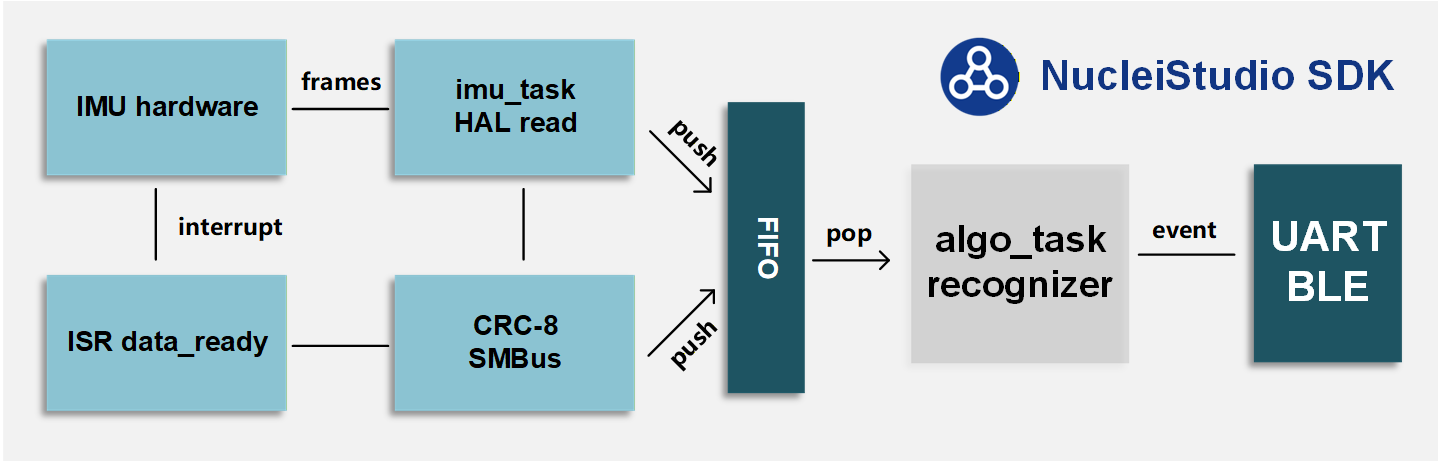
\includegraphics[width=\textwidth]{fig_software_flow.png}
    \caption{系统软件架构总览。IMU硬件通过中断触发imu\_task进行数据读取和CRC计算，样本通过FIFO传递至algo\_task进行手势识别，识别结果通过UART输出并可由BLE服务推送。}
    \label{fig:overview_arch}
\end{figure*}

系统运行在RISC-V nuclei\_evalsoc处理器上，使用FreeRTOS实时操作系统进行任务调度\cite{freertos,nuclei_sdk}。芯原VPI事件系统负责模块间消息传递。VPI的全称为VeriSilicon Platform Interface，用于连接中断服务程序与任务、任务与任务之间的异步流程。

核心数据链路如下：IMU硬件产生数据就绪中断，服务程序通过VPI通知\texttt{imu\_task}；\texttt{imu\_task}经HAL接口读取FIFO数据、更新CRC校验并将样本写入共享FIFO；随后VPI通知\texttt{algo\_task}，由算法任务完成滑动窗口管理、特征提取、分类推理和状态机决策；检测到手势后，系统通过UART输出结果并更新BLE服务。整条链路可在一个IMU采样周期内完成，采样周期为20~ms。

\subsection{平台规格与约束}

目标平台的关键参数如表~\ref{tab:platform_spec}所示。

\begin{table}[htbp]
    \centering
    \caption{目标平台硬件规格}
    \label{tab:platform_spec}
    \begin{tabular}{ll}
        \toprule
        \textbf{参数} & \textbf{规格} \\
        \midrule
        处理器架构     & RISC-V nuclei\_evalsoc \\
        Flash容量     & 3~MB \\
        RAM容量       & 256~KB \\
        操作系统       & FreeRTOS \\
        IMU采样率      & 50~Hz，6轴同步采集 \\
        陀螺仪量程     & $\pm2000$~dps \\
        加速度计量程    & $\pm8$~g \\
        通信接口       & BLE + UART \\
        \bottomrule
    \end{tabular}
\end{table}

在上述硬件约束下，我们的算法需要满足以下设计要求：

\begin{itemize}[leftmargin=*]
    \item 模型参数以\texttt{const float}数组形式存储于Flash中，避免占用RAM。
    \item 推理过程不使用动态内存分配，所有缓冲区在编译时静态确定。
    \item 滑动窗口处理使用环形缓冲区，避免大量数据拷贝。
    \item 单次推理延迟不超过一个采样周期，即20~ms。
\end{itemize}

代码~\ref{lst:recognizer_struct}给出了手势识别器的核心数据结构。该结构体包含滑动窗口环形缓冲区、滤波器状态、分类置信度历史和状态机运行时变量，作为静态全局变量分配，无动态内存开销。

\begin{lstlisting}[caption={手势识别器核心数据结构（gesture\_algorithm.h）},label={lst:recognizer_struct}]
typedef struct GestureRecognizer_st {
    int16_t ring[GESTURE_WINDOW_SIZE][GESTURE_AXIS_COUNT];
    float filter_ring[GESTURE_WINDOW_SIZE]
                     [GESTURE_FILTER_FEATURE_COUNT];
    float filter_low[GESTURE_AXIS_COUNT];
    float filter_high[GESTURE_AXIS_COUNT];
    float filter_mid[GESTURE_AXIS_COUNT];
    float filter_prev[GESTURE_AXIS_COUNT];
    float score_history[8][7];
    uint16_t write_pos;
    uint16_t sample_count;
    uint16_t stride_count;
    uint32_t total_samples;
    uint8_t score_history_pos;
    uint8_t score_history_count;
    bool filter_initialized;
    GestureLabel run_label;
    uint8_t run_count;
    uint8_t small_count;
    bool small_wait_idle;
    uint8_t small_idle_count;
    float small_pinch_sum;
    float small_clench_sum;
    float small_temporal_pinch_sum;
    float small_temporal_clench_sum;
    uint32_t last_emit_ms;
} GestureRecognizer;
\end{lstlisting}

\subsection{数据集概况}

竞赛提供了VeriHealthi IMU Dataset，数据集的统计信息如表~\ref{tab:dataset_stat}和图~\ref{fig:dataset_dist}所示。

\begin{table}[htbp]
    \centering
    \caption{VeriHealthi IMU数据集统计}
    \label{tab:dataset_stat}
    \begin{tabular}{lccc}
        \toprule
        \textbf{手势类别} & \textbf{录制数量} & \textbf{采集者数量} & \textbf{含标签} \\
        \midrule
        pinch，双指互点 & 154 & 6 & 是 \\
        clench，握拳   & 154 & 6 & 是 \\
        up，抬腕       & 150 & 6 & 是 \\
        down，放下     & 150 & 6 & 是 \\
        others，其他   & 57  & 6 & 否 \\
        \midrule
        \textbf{合计}   & \textbf{665} & \textbf{6} & — \\
        \bottomrule
    \end{tabular}
\end{table}

\begin{figure*}[!t]
    \centering
    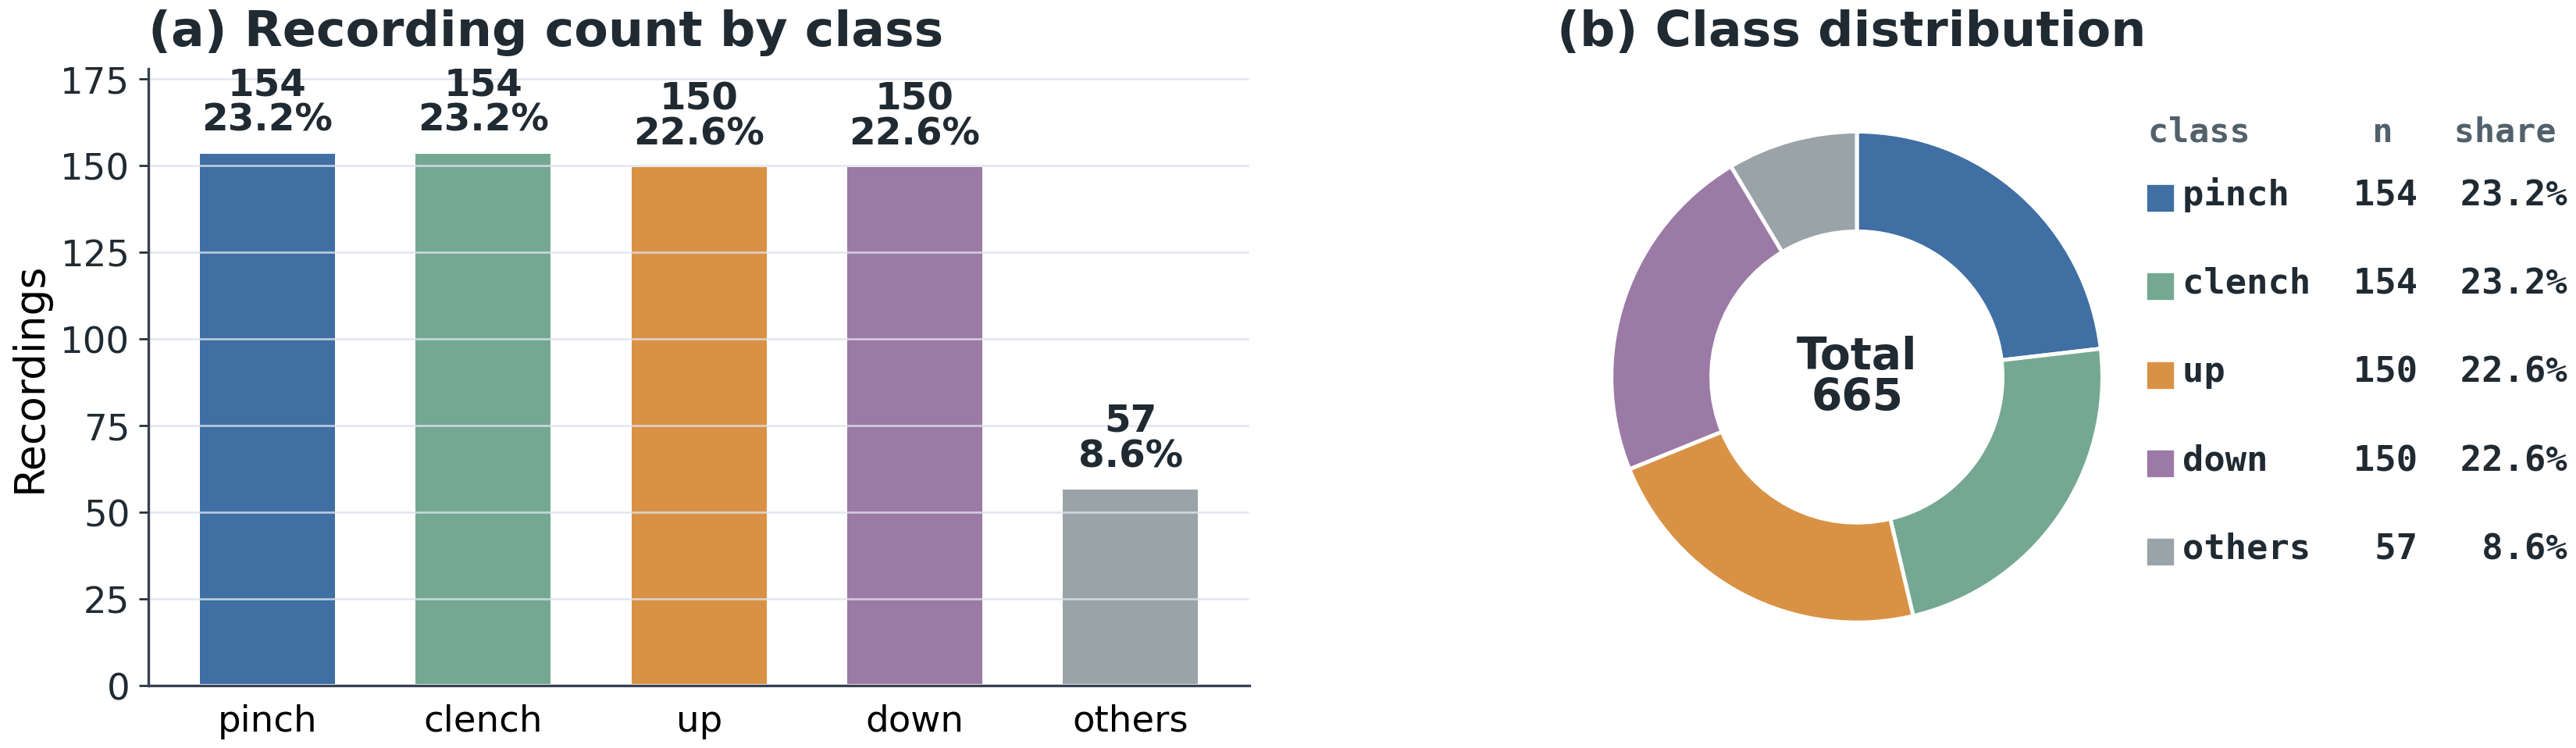
\includegraphics[width=\textwidth]{fig_dataset_dist.png}
    \caption{数据集各类别录制数量分布及占比。四类手势数据相对均衡，others类用于训练负类样本。}
    \label{fig:dataset_dist}
\end{figure*}

如图2中a和b所示，数据集共包含 665 段 IMU 录制，覆盖 pinch、clench、up、down 和 others 五类动作。其中四类目标手势的样本规模较为接近：pinch 和 clench 各 154 段，分别占 23.2\%；up 和 down 各 150 段，分别占 22.6\%。这种分布使模型在四类目标手势上能够获得相对均衡的训练样本，减少由类别数量差异带来的偏置。others 类共有 57 段，占 8.6\%，主要用于表示非目标手势和背景干扰动作，在训练中承担负样本作用，帮助模型降低误触发率。

数据集中每条录制包含一个IMU原始数据文件和一个对应的CSV标签文件。数据来自6位采集者，编号为ID0--ID5，涵盖左手和右手录制。up和down共享同一类录制文件，文件名以\texttt{IMU\_updown\_*}开头，同一段录制中交替包含两种手势事件，需要依据标签文件区分。

数据文件的前5行为元信息头，从第6行开始为7列数值数据，其中第1列为序列号，第2--4列为陀螺仪原始值，第5--7列为加速度计原始值。

\subsection{评估指标}

竞赛采用基于事件窗口匹配的F1评估方法。对于每个标注事件，系统需要在事件发生时间前0.3秒到事件发生时间之间输出正确类别，才记为真正例。真正例、假正例和假负例分别记为TP、FP和FN。评估指标包括：

\begin{itemize}[leftmargin=*]
    \item \textbf{Precision}：精确率，$P = \mathrm{TP} / (\mathrm{TP} + \mathrm{FP})$
    \item \textbf{Recall}：召回率，$R = \mathrm{TP} / (\mathrm{TP} + \mathrm{FN})$
    \item \textbf{F1 Score}：F1分数，$F_1 = 2PR / (P + R)$
    \item \textbf{Macro F1}：宏平均F1，四类手势F1的算术平均
\end{itemize}

此外，系统需要在QEMU回放开始后输出CRC-8/SMBus校验值。该值对IMU原始数据前320000字节计算，用于验证数据读取顺序和字节处理逻辑。竞赛评估采用固定的QEMU测试序列，详见第\ref{sec:results}节。该序列由多位用户的多段录制拼接而成，总计87个标注手势事件。

% ============================================================
\section{算法设计}
\label{sec:algorithm}
% ============================================================

本节介绍数据预处理、特征工程、分类推理和状态机决策逻辑。算法先用全局网络给出候选类别，再对容易混淆的小手势进行二分类和时序校验，最后由状态机输出事件。

\subsection{数据预处理与滑动窗口}

\subsubsection{原始数据格式转换}

IMU硬件返回的原始数据为16位有符号整数（\texttt{int16\_t}），需要转换为物理单位。陀螺仪数据的转换系数为16.4~LSB/dps，加速度计的转换系数为4096~LSB/g。在嵌入式实现中，为了节省RAM和计算开销，统计特征的提取直接使用原始整数值，仅在滤波器组计算时进行物理单位转换。这一设计减少了浮点运算次数，同时保证了特征值的数值稳定性。

\subsubsection{滑动窗口机制}

系统采用固定长度的滑动窗口对连续的IMU数据流进行分帧处理，如图~\ref{fig:sliding_window}所示。

\begin{figure}[htbp]
    \centering
    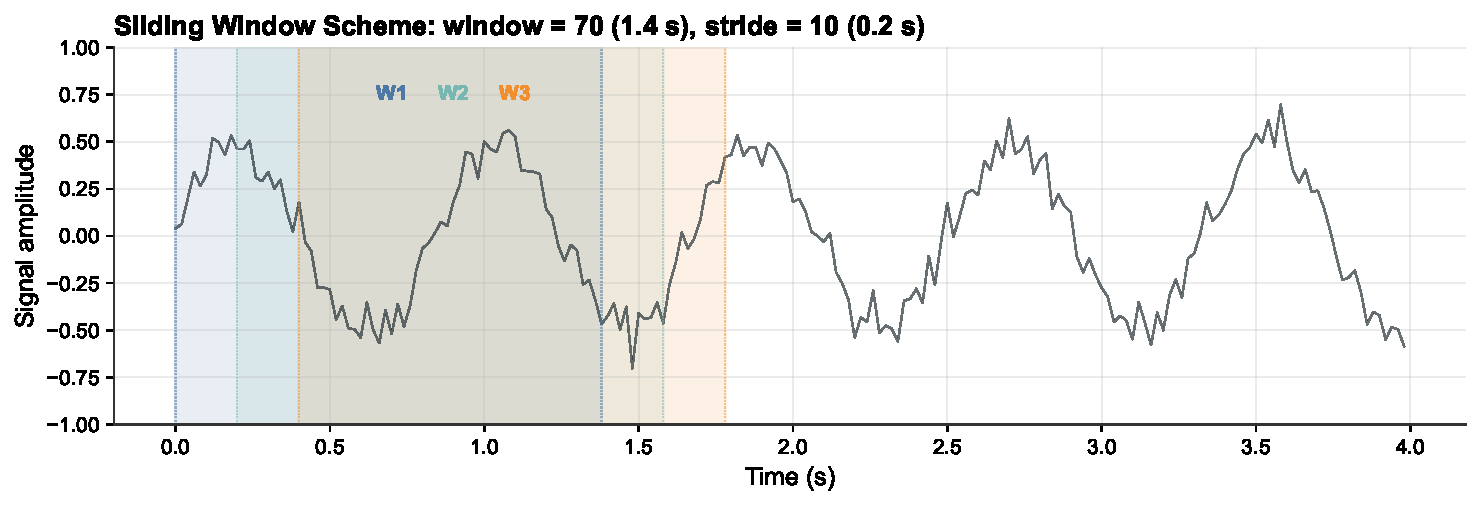
\includegraphics[width=\linewidth]{fig_sliding_window.pdf}
    \caption{滑动窗口分帧示意图。窗口大小为70个采样点，对应1.4秒；步长为10个采样点，对应0.2秒；相邻窗口有85.7\%的重叠。}
    \label{fig:sliding_window}
\end{figure}

窗口参数的设计依据如下：

\begin{itemize}[leftmargin=*]
    \item \textbf{窗口大小}$W = 70$：对应1.4秒数据。该长度覆盖了pinch、clench、up和down的典型持续时间，同时保留足够的统计稳定性。实验比较了50--100个采样点的窗口，70个采样点在检测精度和响应延迟之间较为均衡。
    \item \textbf{步长}$S = 10$：对应0.2秒数据。系统每0.2秒产生一次推理输出，状态机可以得到足够密集的决策信息。相邻窗口之间有$60/70 = 85.7\%$的重叠，有利于平滑时间维度上的类别变化。
\end{itemize}

在嵌入式实现中，滑动窗口通过环形缓冲区管理。\texttt{GestureRecognizer}结构体中包含$70 \times 6$的\texttt{int16\_t}数组\texttt{ring}，用于存储原始IMU数据；另有$70 \times 4$的\texttt{float}数组\texttt{filter\_ring}，用于存储滤波器特征。写入位置由\texttt{write\_pos}追踪，每收到一个新样本后递增并取模。当\texttt{sample\_count}达到窗口大小$W$后，每隔$S$个样本触发一次特征提取与推理。

环形缓冲区的使用避免了每次窗口滑动时对整个窗口数据的拷贝操作。特征提取时，通过合理的索引计算，从环形缓冲区中直接读取当前窗口对应的数据，实现了$O(1)$的窗口滑动开销。

\subsection{特征工程}

本方案使用85维特征向量，由77维统计特征和8维滤波器组特征组成。前者提供了可解释的时域统计描述，后者引入了频域分量的判别信息。

\subsubsection{77维统计特征}

一个滑动窗口包含6条同步信号，分别为三轴陀螺仪$g_x$、$g_y$、$g_z$和三轴加速度计$a_x$、$a_y$、$a_z$。统计特征的设计从单轴幅度开始：均值、标准差、峰值、能量和过零率描述每条轴在窗口内的基本变化。随后加入轴间相关系数，用来刻画手腕旋转时多轴之间的协同变化。对于up和down这类大幅度动作，单轴统计量容易受佩戴方向影响，因此进一步计算合加速度和合角速度。对于pinch和clench这类小手势，仅看幅度不足以稳定区分，还需要加入加速度与角速度之间的相对强弱以及分布宽度。最终得到表~\ref{tab:stat_features}中的77维统计特征。

\begin{table}[htbp]
    \centering
    \caption{77维统计特征构成}
    \label{tab:stat_features}
    \begin{tabular}{lcp{4.5cm}}
        \toprule
        \textbf{特征类型} & \textbf{维度} & \textbf{说明} \\
        \midrule
        均值 mean        & 6   & 各轴信号均值 \\
        标准差 std       & 6   & 各轴信号波动程度 \\
        最大值 max       & 6   & 各轴信号峰值 \\
        最小值 min       & 6   & 各轴信号谷值 \\
        峰峰值 range     & 6   & max$-$min，信号动态范围 \\
        能量 energy      & 6   & $\sum x_i^2 / N$，信号强度 \\
        过零率 ZCR       & 6   & 信号穿越零点的频率 \\
        绝对均值 abs mean & 6   & $\sum |x_i| / N$ \\
        轴间相关 corr    & 15  & $\binom{6}{2}$个轴对的Pearson相关系数 \\
        合加速度均值        & 1   & $\overline{\sqrt{a_x^2 + a_y^2 + a_z^2}}$ \\
        合加速度标准差      & 1   & $\mathrm{std}(\sqrt{a_x^2 + a_y^2 + a_z^2})$ \\
        合角速度均值        & 1   & $\overline{\sqrt{g_x^2 + g_y^2 + g_z^2}}$ \\
        合角速度标准差      & 1   & $\mathrm{std}(\sqrt{g_x^2 + g_y^2 + g_z^2})$ \\
        加速度与陀螺仪比值  & 6   & 三轴$r_i=|a_i|/(|g_i|+\epsilon)$的均值和最大值 \\
        四分位距 IQR     & 4   & $Q_{75}-Q_{25}$，描述中间50\%样本跨度 \\
        \midrule
        \textbf{合计}       & \textbf{77} & — \\
        \bottomrule
    \end{tabular}
\end{table}


这里的$x_i$表示某一通道在窗口内的第$i$个采样点，$N=70$为窗口长度。$a_i$和$g_i$在比值特征中表示同一坐标轴上的加速度和角速度幅值，$i\in\{x,y,z\}$；$\epsilon$是很小的正数，用于避免角速度接近零时出现除零。四分位距IQR的英文全称为Interquartile Range，其中$Q_{25}$为第25百分位数，$Q_{75}$为第75百分位数。IQR只关注排序后中间一半样本的跨度，比最大值和最小值更不容易受孤立尖峰影响。

嵌入式实现中，统计特征采用单遍扫描计算。遍历窗口数据时同步维护运行和与运行平方和，可同时得到均值、标准差和能量等统计量，避免多次遍历窗口。四分位距IQR使用选择算法直接寻找第25和第75百分位数，时间复杂度为$O(N)$。

\subsubsection{8维滤波器组特征}

参考文献\cite{xu2022enabling}中的信号分解方法，本方案设计了一组单极点IIR滤波器，将IMU信号分解为低频趋势、高频分量和中频手势分量。中频分量约为8--20~Hz，与手指和手腕运动的主要频段相近，携带较多判别信息。

记$\mathbf{x}[n]\in\mathbb{R}^{6}$为第$n$个六轴IMU采样点，三个陀螺仪轴和三个加速度计轴按同一递推公式逐元素计算。$\mathbf{l}[n]$、$\mathbf{h}[n]$和$\mathbf{m}[n]$分别表示低通输出、高通输出和中频输出，它们都是6维向量；$\mathbf{x}[n-1]$为上一采样点，$\mathbf{l}[n-1]$、$\mathbf{h}[n-1]$、$\mathbf{m}[n-1]$为上一时刻的滤波器状态。滤波器组的递推形式如下：

\textbf{低通滤波器，等效截止频率7.99~Hz}：
\begin{equation}
    \mathbf{l}[n] = \mathbf{l}[n-1] + \alpha_\mathrm{LP} \cdot (\mathbf{x}[n] - \mathbf{l}[n-1])
\end{equation}
其中$\alpha_\mathrm{LP} = 0.5010$为低通滤波系数。该式等价于指数滑动平均：当前输入$\mathbf{x}[n]$与上一低通状态$\mathbf{l}[n-1]$的差值先乘以$\alpha_\mathrm{LP}$，再累加到上一状态上。在$f_s=50$~Hz时对应$f_c=7.9896$~Hz。该分支用于保留手臂姿态和慢速握拳带来的低频趋势。

\textbf{高通滤波器，等效截止频率8.02~Hz}：
\begin{equation}
    \mathbf{h}[n] = \alpha_\mathrm{HP} \cdot (\mathbf{h}[n-1] + \mathbf{x}[n] - \mathbf{x}[n-1])
\end{equation}
其中$\alpha_\mathrm{HP} = 0.4980$为高通滤波系数。括号内的$\mathbf{x}[n]-\mathbf{x}[n-1]$描述相邻采样点的变化量，上一高通状态$\mathbf{h}[n-1]$用于保持递推连续性。按照一阶RC离散化关系$f_c=f_s(1-\alpha)/[2\pi\alpha]$反推，在$f_s=50$~Hz时对应$f_c=8.0217$~Hz。该滤波器会削弱缓慢变化的姿态趋势，保留短时间内快速变化的部分，适合捕捉pinch触碰瞬间产生的细小振动。

\textbf{中频带通滤波器，通带约8.02--20.00~Hz}：
\begin{equation}
    \mathbf{m}[n] = \mathbf{m}[n-1] + \alpha_\mathrm{BP} \cdot (\mathbf{h}[n] - \mathbf{m}[n-1])
\end{equation}
其中$\alpha_\mathrm{BP} = 0.7154$为带通低通系数。对高通输出$\mathbf{h}[n]$再做一次低通平滑；按同一系数关系反推，该级低通等效截止频率为20.0034~Hz。经过前级高通和本级低通后，剩余部分主要落在8.02--20.00~Hz附近，因此记为中频分量$\mathbf{m}[n]$。


\begin{figure*}[!t]
    \centering
    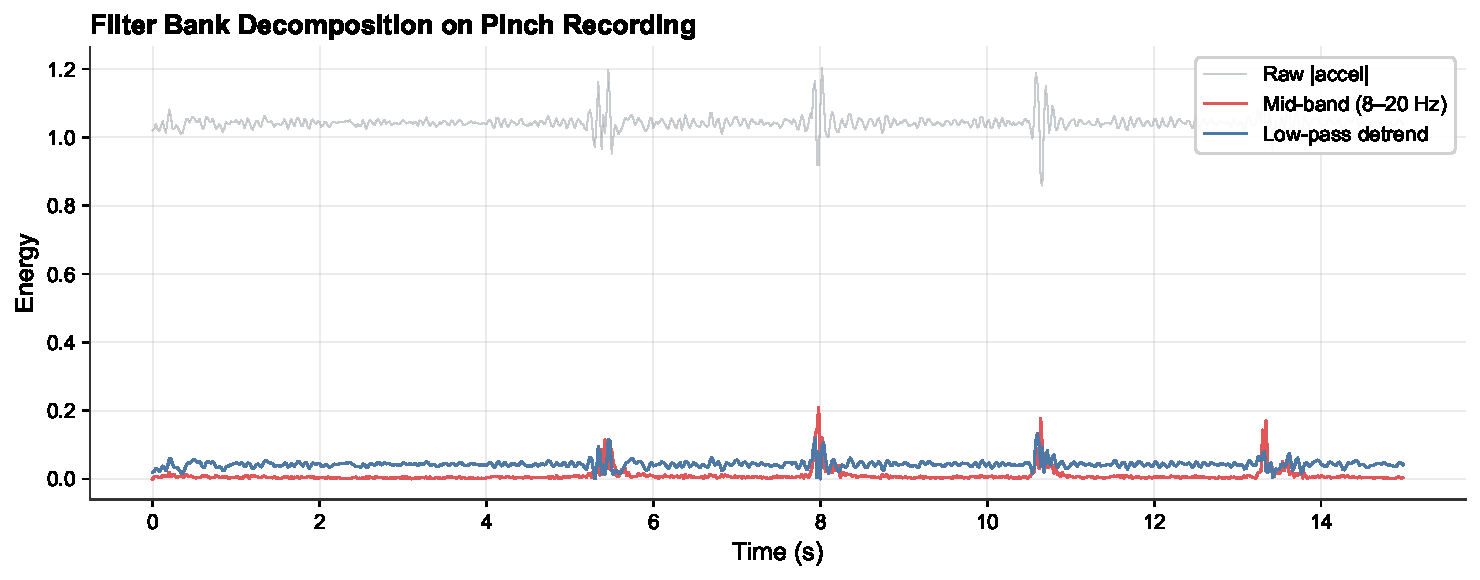
\includegraphics[width=\textwidth]{fig_filter_bank.pdf}
    \caption{滤波器组在pinch录制上的分解效果。中频分量约为8--20~Hz，能够反映手指微小运动产生的周期性信号模式。}
    \label{fig:filter_bank}
\end{figure*}

从每个时刻的滤波器输出中提取4个标量特征：

\begin{enumerate}[leftmargin=*]
    \item $\|\mathbf{m}_\mathrm{gyro}\|_2$：中频陀螺仪能量——反映手指/手腕微小运动产生的中频旋转信号
    \item $\|\mathbf{m}_\mathrm{accel}\|_2$：中频加速度计能量——反映手指/手腕微小运动产生的中频线性加速度
    \item $\|\mathbf{l}_\mathrm{gyro}\|_2$：低通陀螺仪能量——反映手臂的缓慢旋转趋势
    \item $|\|\mathbf{l}_\mathrm{accel}\|_2 - 1|$：低通加速度计去重力偏差，用于反映手臂姿态偏移
\end{enumerate}

对滑动窗口内的4个滤波器特征序列分别计算均值和最大值，得到$4 \times 2 = 8$维滤波器组特征。pinch主要表现为手指微小运动产生的中高频振动；up和down伴随手臂大幅运动；clench则更多体现为握拳时的慢速肌肉收缩。频段分解有助于区分这三类运动形态。

图~\ref{fig:filter_bank}展示了滤波器组在pinch录制上的分解效果。手势发生时段的中频能量升高，低通去趋势分量则对应手臂姿态的缓慢变化。

滤波器组采用流式计算模式。每收到一个新的IMU样本，系统更新低通、高通、中频和上一样本状态，并将当前时刻的4个标量特征写入\texttt{filter\_ring}。该实现避免了在特征提取阶段重新遍历窗口数据，滤波器更新开销为$O(1)$。

\subsection{原始IMU信号分析}

频域特征和状态机策略的设计来自原始IMU信号的差异，图~\ref{fig:raw_imu}--图~\ref{fig:updown_waveform}给出了典型录制的波形和幅度对比。从幅度和频率两方面看，pinch和clench都属于小手势，但二者仍存在差别：pinch更接近短促振动，clench更接近中等幅度的慢速变化。up和down则伴随前臂旋转，陀螺仪和加速度计幅度均明显更大。others类没有稳定形态，包含走路、摆臂和日常手部活动。

\begin{figure*}[!t]
    \centering
    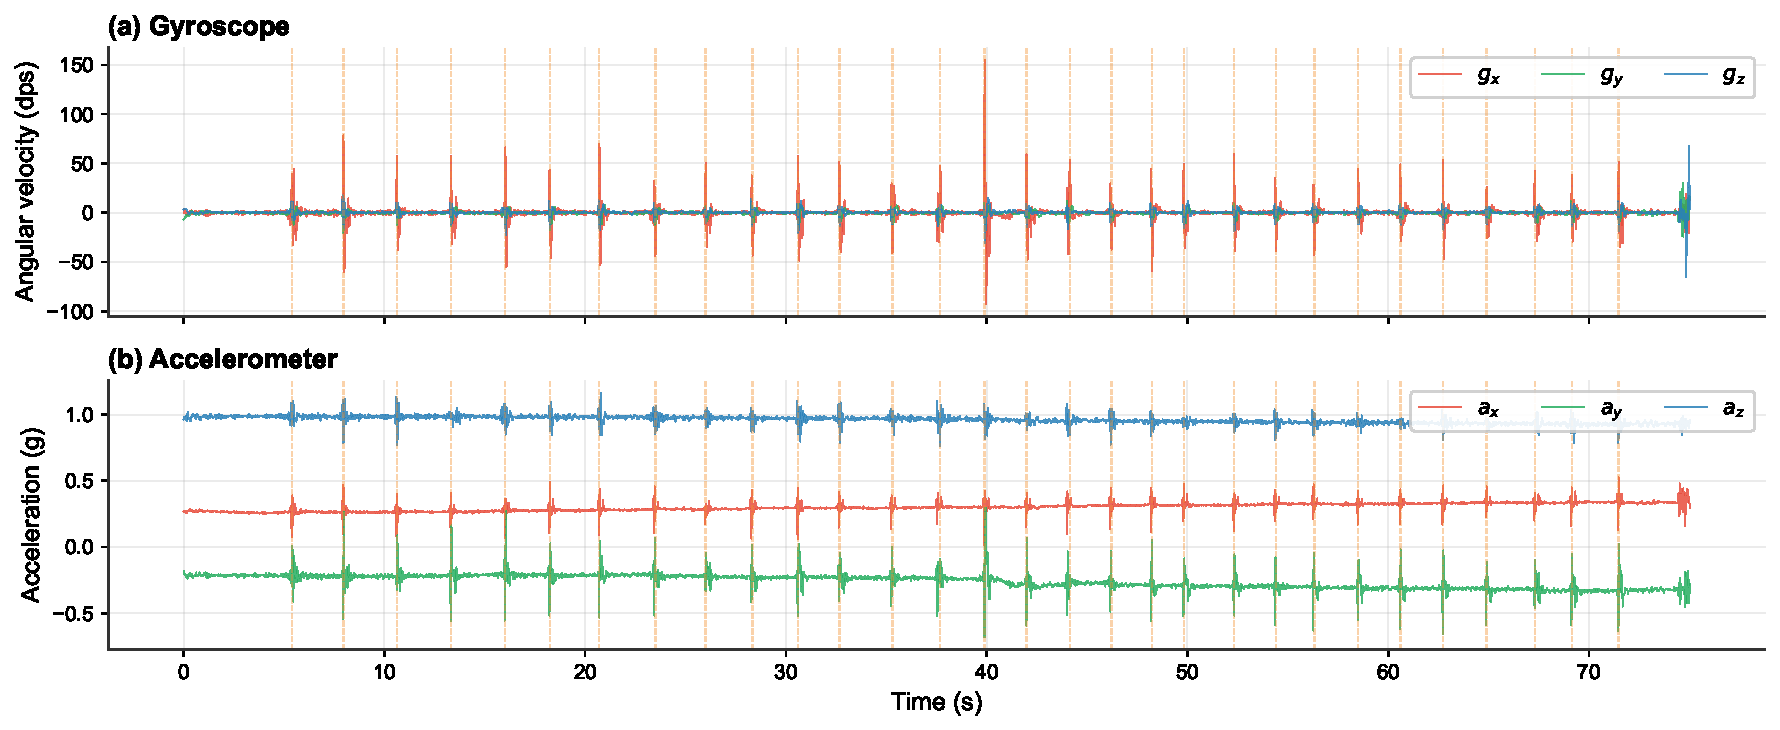
\includegraphics[width=\textwidth]{fig_raw_imu_pinch.pdf}
    \caption{Pinch录制的原始IMU 6轴波形。上：陀螺仪三轴角速度；下：加速度计三轴加速度。橙色虚线为标注的手势事件时间点。}
    \label{fig:raw_imu}
\end{figure*}

\begin{figure}[!t]
    \centering
    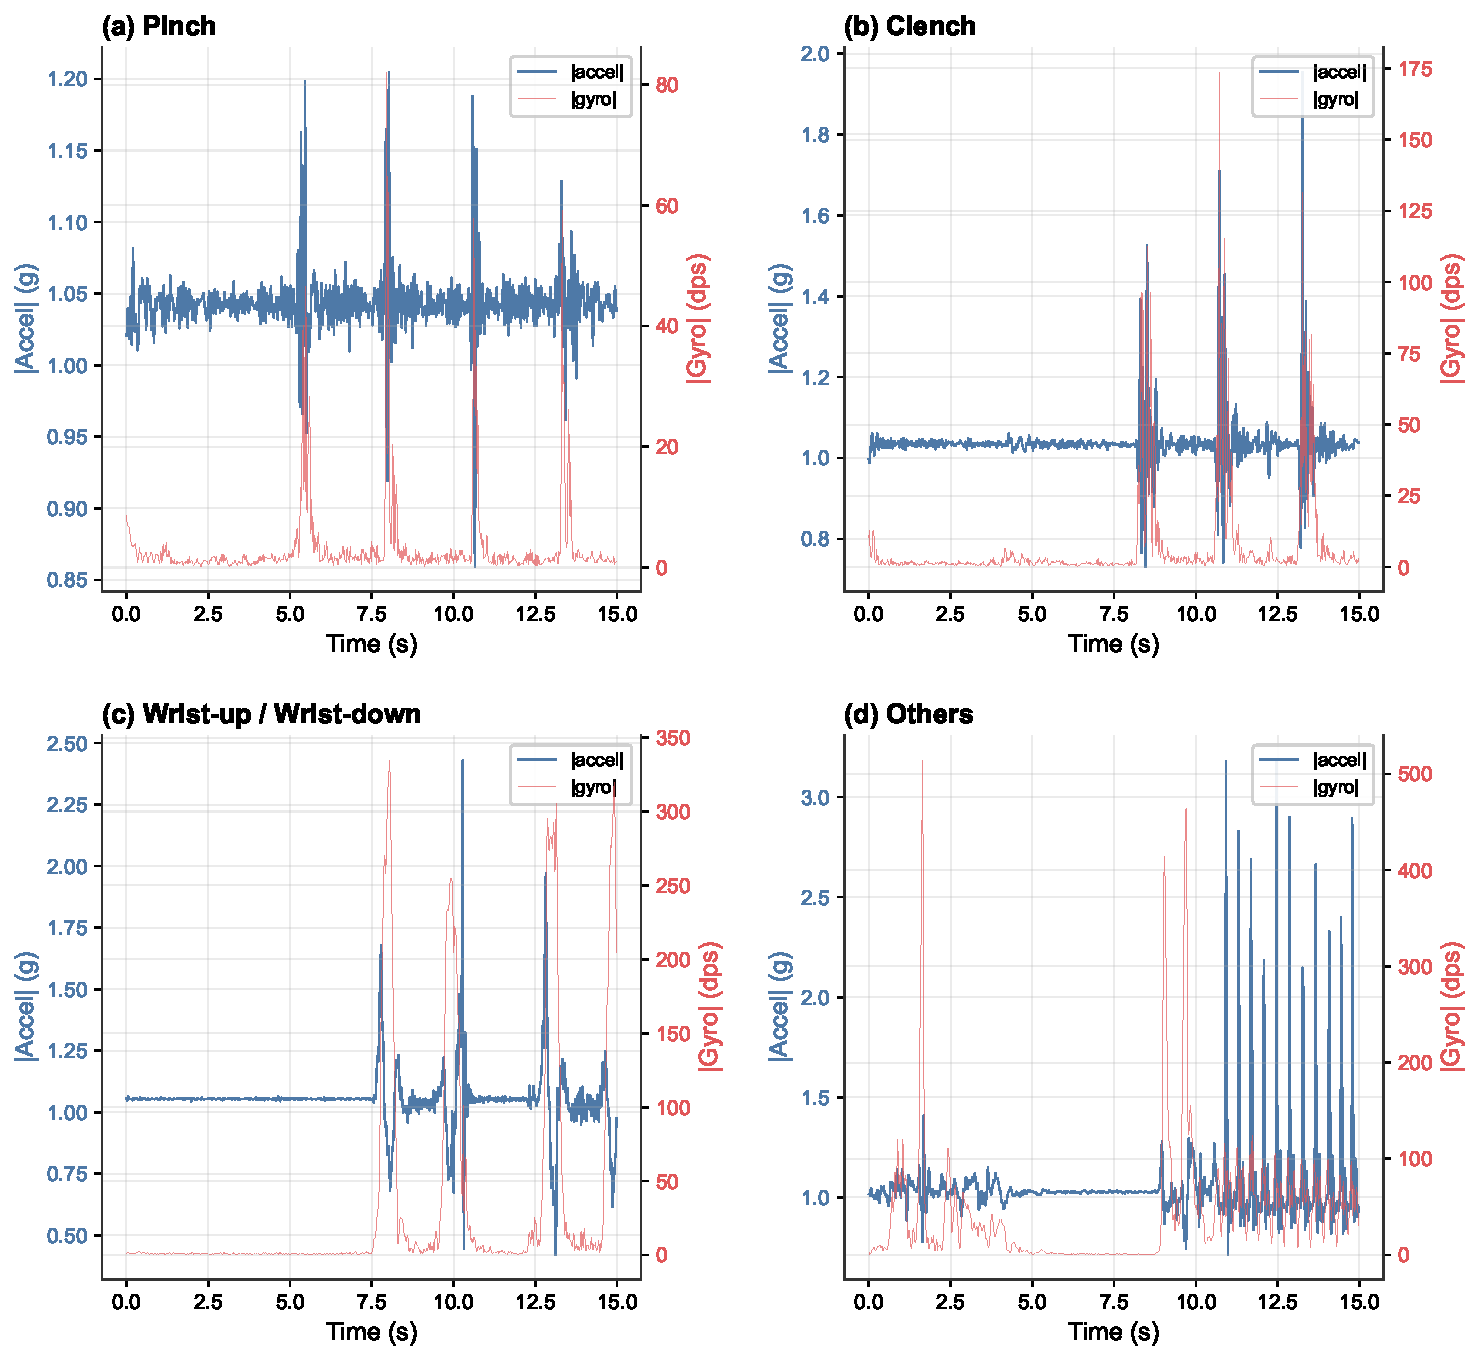
\includegraphics[width=\columnwidth]{fig_four_gestures.pdf}
    \caption{四类手势的IMU信号幅度对比。pinch：微弱高频振动；clench：中等幅度慢速变化；up/down：大幅度手臂旋转信号；others：随机运动模式。}
    \label{fig:four_gestures}
\end{figure}

\begin{figure}[!t]
    \centering
    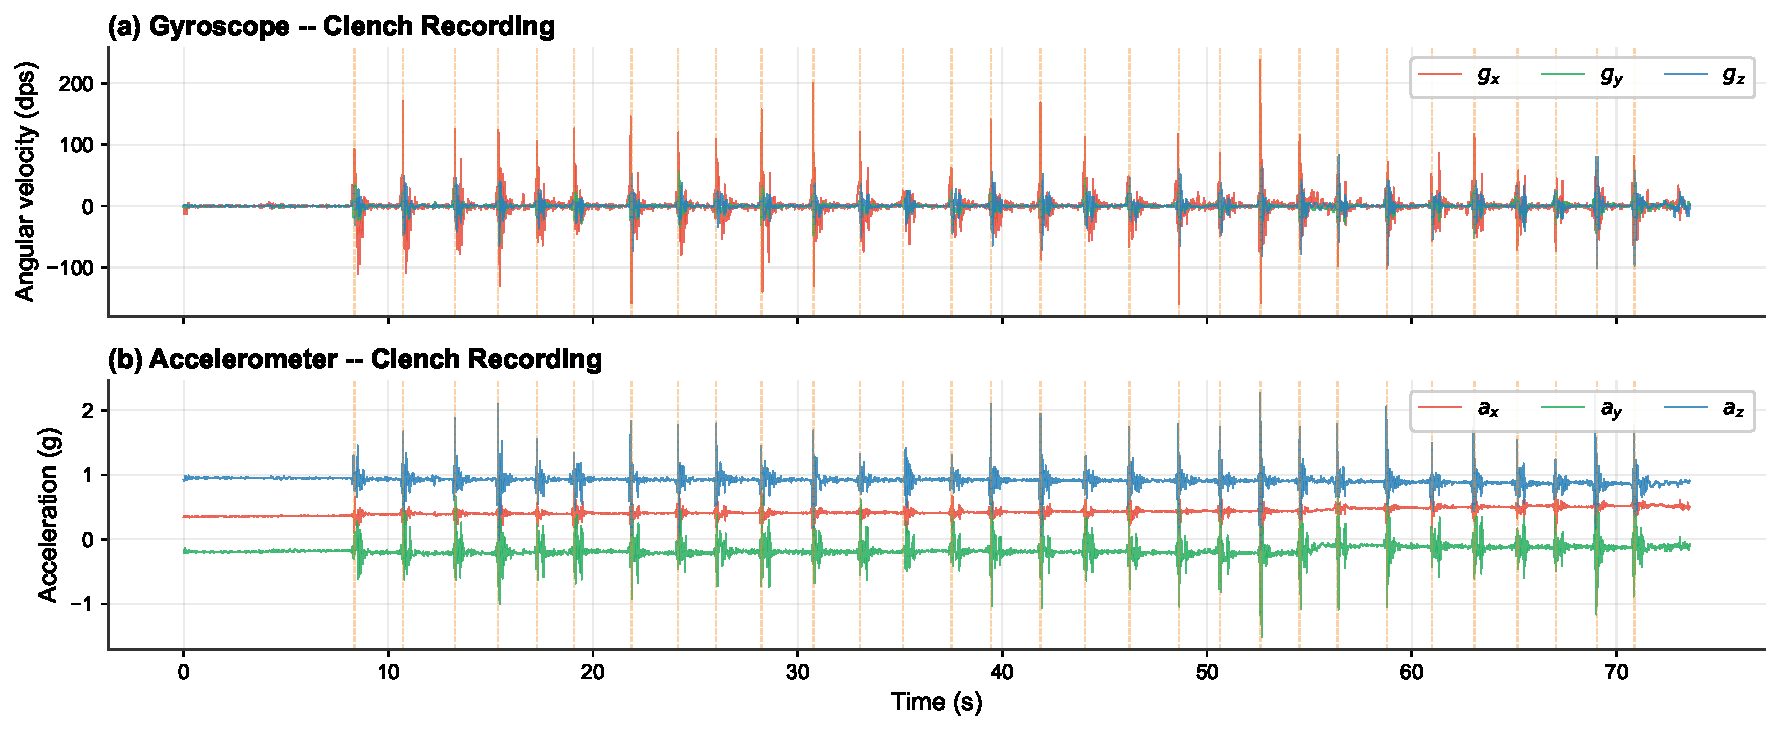
\includegraphics[width=\columnwidth]{fig_clench_waveform.pdf}
    \caption{Clench录制的原始IMU 6轴波形。握拳动作在加速度计上产生中等幅度的信号变化，陀螺仪响应相对较弱。}
    \label{fig:clench_waveform}
\end{figure}

\begin{figure}[!t]
    \centering
    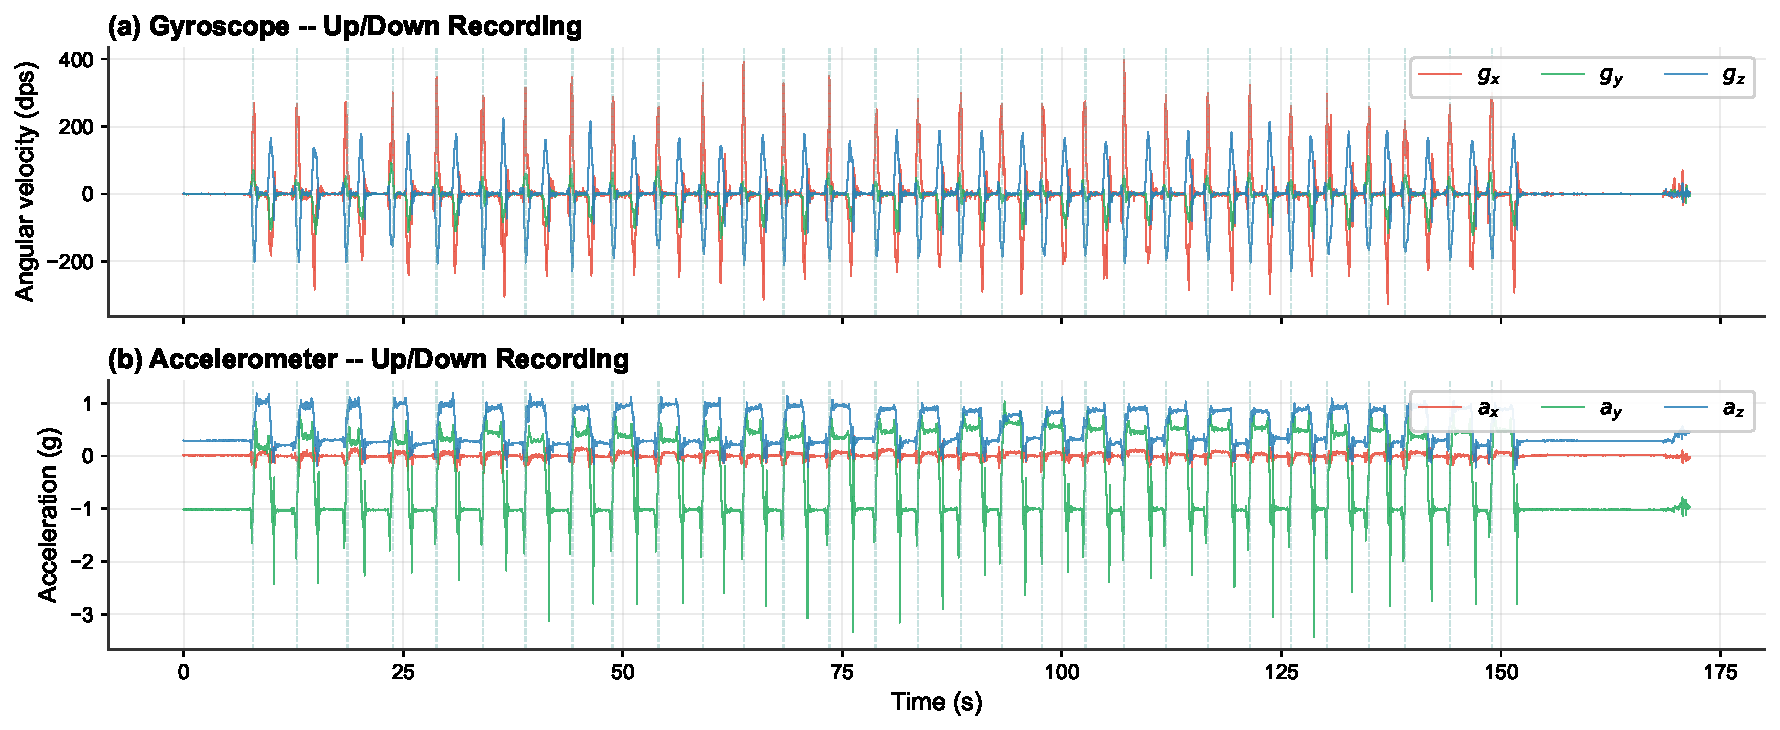
\includegraphics[width=\columnwidth]{fig_updown_waveform.pdf}
    \caption{Up/down录制的原始IMU 6轴波形。手臂旋转动作在陀螺仪和加速度计上均产生大幅度的特征信号。}
    \label{fig:updown_waveform}
\end{figure}

综合原始波形可以看到，四类动作不仅幅度大小不同，频率范围、持续时间和事件间隔也存在差异。pinch的主要线索是短促高频分量，clench更依赖中低频幅度变化，up/down则表现为连续的大幅旋转。后续分类框架据此采用“窗口特征判别+短时序列校验+状态机聚合”的结构：窗口特征负责给出当前片段的候选类别，时序校验检查多个窗口的一致性，状态机再把连续窗口转化为最终事件。


\subsection{分类推理框架}

\begin{figure*}[!t]
    \centering
    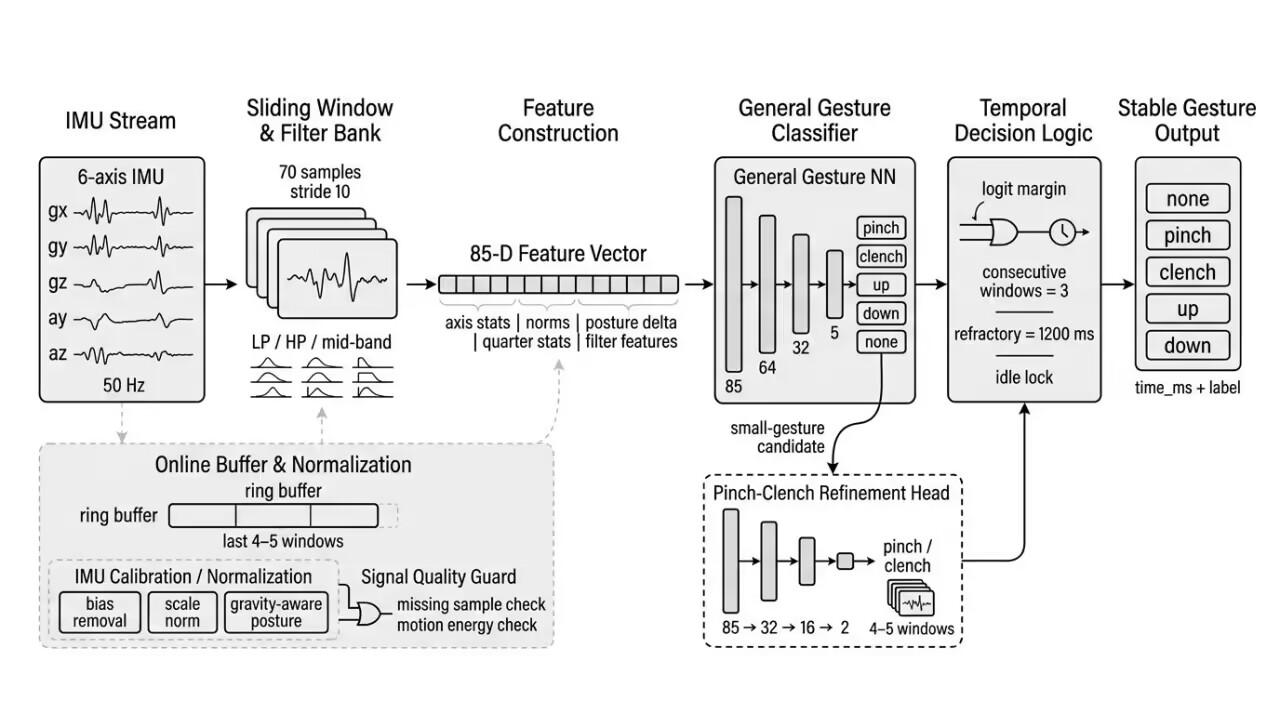
\includegraphics[width=\textwidth]{fig_nn_architecture.png}
    \caption{分类推理流程图。85维特征首先进入全局五分类网络和pinch/clench二分类网络，随后由短时序列校验和模板距离校验补充判别信息，最终由状态机输出手势事件。}
    \label{fig:nn_arch}
\end{figure*}

特征提取完成后，算法并不直接用单个窗口给出事件，而是先得到几个互补的判别量，再交给状态机做事件级输出。全局五分类网络负责回答“当前窗口最像哪一类”，pinch/clench二分类网络负责回答“小手势内部更像双指互点还是握拳”，短时序列校验负责判断最近多个窗口是否在时间上连续，质心距离校验负责排除偏离训练样本分布的异常小手势。推理流程如图~\ref{fig:nn_arch}所示。

\subsubsection{全局五分类网络}

下面先给出统一符号。$\mathbf{f}\in\mathbb{R}^{85}$表示标准化后的85维特征向量；$\mathbf{W}$和$\mathbf{b}$分别表示神经网络的权重矩阵和偏置向量，训练完成后以\texttt{const float}数组固化到Flash。$\mathrm{ReLU}(u)=\max(u,0)$为激活函数。网络输出记为logit，logit是softmax之前的原始类别分数，数值越大表示该类越可能被选中。全局网络输出$\mathbf{z}_\mathrm{NN}$的5个分量按$[\mathrm{none}, \mathrm{pinch}, \mathrm{clench}, \mathrm{up}, \mathrm{down}]$排列，其中NN表示Neural Network；二分类网络输出$\mathbf{z}_\mathrm{PC}$的2个分量按$[\mathrm{pinch}, \mathrm{clench}]$排列，其中PC表示pinch/clench。

全局五分类网络是主干分类器，对none、pinch、clench、up和down进行初步判别。网络结构为三层多层感知机，英文为Multi-Layer Perceptron，简称MLP：

\begin{equation}
    \begin{aligned}
        \mathbf{h}_1 &= \mathrm{ReLU}(\mathbf{W}_1 \mathbf{f} + \mathbf{b}_1), \quad \mathbf{h}_1 \in \mathbb{R}^{64} \\
        \mathbf{h}_2 &= \mathrm{ReLU}(\mathbf{W}_2 \mathbf{h}_1 + \mathbf{b}_2), \quad \mathbf{h}_2 \in \mathbb{R}^{32} \\
        \mathbf{z}_\mathrm{NN} &= \mathbf{W}_3 \mathbf{h}_2 + \mathbf{b}_3, \quad \mathbf{z}_\mathrm{NN} \in \mathbb{R}^{5}
    \end{aligned}
\end{equation}

式中$\mathbf{h}_1$和$\mathbf{h}_2$是隐藏层特征，维度分别为64和32；$\mathbf{z}_\mathrm{NN}\in\mathbb{R}^{5}$是五分类logit向量。对应的矩阵维度为$\mathbf{W}_1\in\mathbb{R}^{64\times85}$、$\mathbf{W}_2\in\mathbb{R}^{32\times64}$、$\mathbf{W}_3\in\mathbb{R}^{5\times32}$。推理时先对原始85维特征做z-score标准化：
\begin{equation}
    \mathbf{f} = (\mathbf{f}_\mathrm{raw} - \boldsymbol{\mu}) \odot \boldsymbol{\sigma}^{-1}
\end{equation}
其中$\mathbf{f}_\mathrm{raw}$为未标准化特征，$\boldsymbol{\mu}$为训练集均值，$\boldsymbol{\sigma}^{-1}$为标准差倒数，$\odot$表示逐元素乘法。标准化参数在训练阶段计算并固化于Flash中。

全局网络的候选类别由$\arg\max_k z_{\mathrm{NN},k}$给出。若最大分量对应up或down，状态机会进入大手势连续确认路径；若对应pinch或clench，则进入小手势聚合路径，后续还需要二分类网络、时序校验和模板校验共同参与判断。

训练细节如下：
\begin{itemize}[leftmargin=*]
    \item \textbf{优化器}：Adam，学习率$10^{-3}$，权重衰减$10^{-4}$
    \item \textbf{损失函数}：带类别权重的交叉熵损失，权重按类别频率的倒数计算并归一化
    \item \textbf{训练数据构建}：使用全部录制的特征数据，负类none每3个窗口保留1个样本以缓解类别不平衡
    \item \textbf{训练轮数}：60个epoch，batch size为512
    \item \textbf{随机种子}：固定为20260607，保证训练过程可复现
\end{itemize}

全局分类网络的参数量为$85 \times 64 + 64 + 64 \times 32 + 32 + 32 \times 5 + 5 = 7,781$个浮点数，占用Flash空间约31.1~KB。网络隐藏层使用ReLU激活函数，输出层直接给出5类logit值。本文采用MLP而非卷积神经网络或循环神经网络，原因是85维输入已经包含统计和频域信息，MLP可以完成特征到类别的映射，同时推理仅涉及矩阵乘法和逐元素运算，便于在带单精度FPU的RISC-V平台上运行。

\subsubsection{pinch/clench二分类网络}

pinch和clench在幅度上都属于小手势，单靠全局五分类网络容易在二者之间产生混淆。因此，算法对小手势候选再运行一个二分类网络。该网络的输入仍是同一个$\mathbf{f}$，但训练样本只包含pinch和clench两类：

\begin{equation}
    \begin{aligned}
        \mathbf{h}_1^\mathrm{PC} &= \mathrm{ReLU}(\mathbf{W}_1^\mathrm{PC} \mathbf{f} + \mathbf{b}_1^\mathrm{PC}), \quad \mathbf{h}_1^\mathrm{PC} \in \mathbb{R}^{32} \\
        \mathbf{h}_2^\mathrm{PC} &= \mathrm{ReLU}(\mathbf{W}_2^\mathrm{PC} \mathbf{h}_1^\mathrm{PC} + \mathbf{b}_2^\mathrm{PC}), \quad \mathbf{h}_2^\mathrm{PC} \in \mathbb{R}^{16} \\
        \mathbf{z}_\mathrm{PC} &= \mathbf{W}_3^\mathrm{PC} \mathbf{h}_2^\mathrm{PC} + \mathbf{b}_3^\mathrm{PC}, \quad \mathbf{z}_\mathrm{PC} \in \mathbb{R}^{2}
    \end{aligned}
\end{equation}

上式中，上标$\mathrm{PC}$表示这组参数属于pinch/clench二分类网络。$\mathbf{h}_1^\mathrm{PC}$和$\mathbf{h}_2^\mathrm{PC}$分别为32维和16维隐藏层，$\mathbf{z}_\mathrm{PC}\in\mathbb{R}^{2}$为二分类logit向量。$z_{\mathrm{PC},0}$对应pinch，$z_{\mathrm{PC},1}$对应clench。该网络只在全局网络给出小手势候选时参与决策；若全局网络输出up、down或none，二分类结果不会改变当前窗口类别。

二分类网络采用32-16-2结构，小于全局网络的64-32-5结构。二分类任务的边界更集中，不需要同等规模的模型容量。该网络独立训练，输入仍为85维特征，训练样本仅来自pinch和clench两类。

二分类网络的参数量为$85 \times 32 + 32 + 32 \times 16 + 16 + 16 \times 2 + 2 = 3,378$个浮点数，占用Flash约13.5~KB。

为了补偿公开训练集中clench被误分为pinch的错误模式，推理时对clench对应的二分类logit加入一个固定偏置$\beta_\mathrm{clench}=4.0$：

\begin{equation}
    z_\mathrm{PC,clench}' = z_\mathrm{PC,clench} + \beta_\mathrm{clench}
\end{equation}

偏置只作用在二分类网络的clench分量上，不改变全局五分类网络对up和down的判断。小手势聚合结束时，状态机会比较累计后的pinch得分和clench得分，偏置后的$z_\mathrm{PC,clench}'$参与clench累计得分。

\subsubsection{短时序列校验网络}

单帧分类容易受到瞬态噪声影响，尤其在手势起始和结束阶段，局部特征可能接近静止状态或其他手势。为此，本方案使用一个轻量级时序卷积网络对最近8个窗口的logit序列进行建模\cite{bai2018empirical}。时序卷积网络的英文为Temporal Convolutional Network，简称TCN。这里的TCN只做后处理校验，不涉及强化学习。

\begin{equation}
    \begin{aligned}
        \mathbf{s}[t] &= [\mathbf{z}_\mathrm{NN}[t];\; \mathbf{z}_\mathrm{PC}[t]] \in \mathbb{R}^{7} \\
        \mathbf{S} &= [\mathbf{s}[t-7], \ldots, \mathbf{s}[t]] \in \mathbb{R}^{8 \times 7}
    \end{aligned}
\end{equation}

其中$t$表示当前推理窗口的序号，$\mathbf{s}[t]$把当前窗口的5维全局logit和2维二分类logit拼接为7维向量。$\mathbf{S}$为最近8个窗口的logit历史，第一维是时间，第二维是类别分数。8个窗口对应约1.6秒历史，可为状态机提供时间一致性信息。

TCN采用两层因果一维卷积，核大小$k=3$，隐藏维度为8。因果卷积只使用当前窗口和过去窗口，不使用未来信息，因此可以在线运行：

\begin{equation}
    \begin{aligned}
        \mathbf{H}_1 &= \mathrm{ReLU}(\mathrm{CausalConv1d}(\mathbf{S}, \mathbf{W}_\mathrm{c1})) \in \mathbb{R}^{8 \times 8} \\
        \mathbf{H}_2 &= \mathrm{ReLU}(\mathrm{CausalConv1d}(\mathbf{H}_1, \mathbf{W}_\mathrm{c2})) \in \mathbb{R}^{8 \times 8} \\
        \mathbf{u}_\mathrm{TCN} &= \mathbf{H}_2[8,:] \in \mathbb{R}^{8} \\
        \mathbf{z}_\mathrm{TCN} &= \mathbf{W}_\mathrm{fc} \mathbf{u}_\mathrm{TCN} + \mathbf{b}_\mathrm{fc} \in \mathbb{R}^{5}
    \end{aligned}
\end{equation}

式中$\mathbf{W}_\mathrm{c1}$和$\mathbf{W}_\mathrm{c2}$为两层卷积核参数，$\mathbf{H}_1$和$\mathbf{H}_2$为每个时间位置上的8维隐藏表示。$\mathbf{u}_\mathrm{TCN}$取最后一个时间位置的隐藏向量，即当前窗口在过去7个窗口背景下的时序表示；$\mathbf{W}_\mathrm{fc}$和$\mathbf{b}_\mathrm{fc}$把该表示映射为5维时序校验logit。$\mathbf{z}_\mathrm{TCN}$的类别顺序与$\mathbf{z}_\mathrm{NN}$一致。

短时序列校验主要用于抑制孤立的假脉冲：
\begin{itemize}[leftmargin=*]
    \item 当全局网络在单个窗口突然输出高置信度手势预测，而相邻窗口均为none时，时序校验会降低该手势的有效性。
    \item 当全局网络在多个连续窗口输出一致类别时，时序校验会增强该类别在后续状态机中的权重。
\end{itemize}

时序校验网络训练时采用两类数据增强：
\begin{itemize}[leftmargin=*]
    \item 高斯噪声注入：以标准差0.04和0.08两个级别向输入score序列添加随机噪声，增强模型对logit值波动的鲁棒性
    \item 随机缩放：以0.92--1.08倍的随机因子对输入序列进行缩放，模拟不同置信度水平下的输入变化
\end{itemize}

经数据增强，训练样本扩展为4倍，以缓解小模型在有限训练数据上的过拟合。

训练过程为24个epoch，使用带类别权重的交叉熵损失，随机种子为20260616。该网络的总参数量为$(3 \times 7 \times 8 + 8) + (3 \times 8 \times 8 + 8) + (8 \times 5 + 5) = 413$个浮点数，占用Flash约1.7~KB。

在嵌入式实现中，系统维护一个$8 \times 7$的\texttt{score\_history}环形缓冲区。每次新的全局网络和二分类网络结果到来后，缓冲区写入7个logit值，随后直接在该缓冲区上进行因果卷积计算。

\subsubsection{质心距离模板校验}

神经网络给出的是判别分数，但少数异常窗口可能仍落在错误类别一侧。为此，小手势分支还加入质心距离模板校验。该模块不重新训练复杂模型，而是在训练集上为pinch和clench建立两个特征中心，推理时检查当前样本是否离对应中心过远。

具体实现步骤如下：

\begin{enumerate}[leftmargin=*]
    \item \textbf{特征选择}：从85维特征中选取特定的16个维度，构成模板特征子向量$\mathbf{q} \in \mathbb{R}^{16}$。选择这些维度是因为它们在pinch和clench之间具有较强判别力。
    \item \textbf{独立标准化}：对模板特征进行独立的z-score标准化，使用模板专用的均值和方差参数。
    \item \textbf{质心计算}：分别计算训练集中pinch类和clench类样本标准化后的均值向量，作为类别质心$\mathbf{c}_\mathrm{pinch}$和$\mathbf{c}_\mathrm{clench}$。
    \item \textbf{阈值确定}：对训练集中的每个pinch样本计算到pinch质心的距离，取97.5百分位数作为pinch类的接受阈值$\tau_\mathrm{pinch}$；clench类似。
    \item \textbf{推理时校验}：对候选类别$k$计算距离$d_k=\|\mathbf{q}-\mathbf{c}_k\|_2^2$。若$d_k>\tau_k$，说明当前样本偏离该类训练样本中心，对对应类别logit施加惩罚，降低其被选中的概率。
\end{enumerate}

模板校验模块的参数量较小。两个质心向量、标准化均值、方差倒数和接受阈值合计66个浮点数，占用Flash约0.3~KB。

模板校验模块与神经网络的判别机制不同：神经网络学习非线性决策边界，模板校验模块则用距离度量做异常检测式校验。两者互补，有助于减少单一模型的盲区。

\subsection{决策状态机}

分类网络逐窗口输出logit值，状态机将连续窗口结果转化为离散手势事件，同时抑制重复触发。

\begin{figure*}[!t]
    \centering
    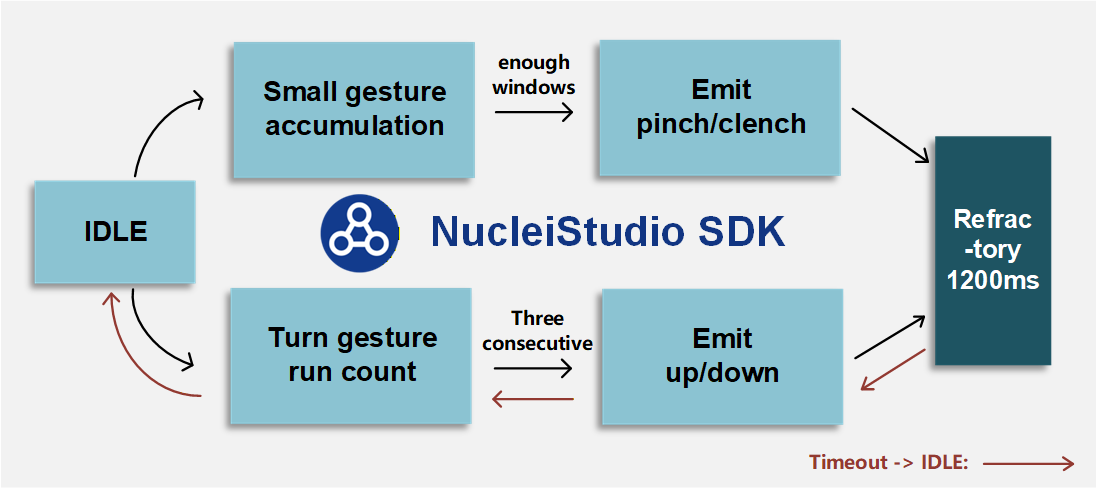
\includegraphics[width=\textwidth]{fig_state_machine.png}
    \caption{手势决策状态机。系统从IDLE状态出发，根据手势类型分别进入小手势聚合路径或大手势连续确认路径，事件输出后进入不应期。}
    \label{fig:state_machine}
\end{figure*}

\subsubsection{小手势与大手势的分类}

算法将四类手势按运动幅度划分为两组，两组手势对应不同的信号特征和检测策略：

\begin{itemize}[leftmargin=*]
    \item \textbf{小手势}：pinch和clench。二者主要由手部微小运动产生，IMU信号幅度较小、持续时间较短，单窗口分类更容易受噪声影响，因此需要多窗口聚合。
    \item \textbf{大手势}：up和down。二者伴随手臂旋转，信号幅度较大、持续时间较长，单窗口分类置信度较高，连续确认即可降低偶发误判。
\end{itemize}

\subsubsection{小手势聚合机制}

对于pinch和clench，系统采用以下聚合策略：

\begin{enumerate}[leftmargin=*]
    \item \textbf{进入条件}：当全局网络输出的最大logit对应pinch或clench，且logit margin超过阈值$\theta_\mathrm{margin} = 2.5$时，进入小手势聚合状态。
    \item \textbf{聚合累加}：在聚合状态中，累加二分类网络的pinch与clench logit，并加入时序校验网络对两类的logit。代码中维护\texttt{small\_pinch\_sum}、\texttt{small\_clench\_sum}、\texttt{small\_temporal\_pinch\_sum}和\texttt{small\_temporal\_clench\_sum}四个变量。
    \item \textbf{退出检测}：聚合过程中，若当前窗口不再是小手势候选，则进入等待空闲状态。在该状态下连续检测到2个none类窗口后，聚合结束。
    \item \textbf{窗口计数确认}：
    \begin{itemize}
        \item 对pinch，需要至少$N_\mathrm{pinch\_first} = 5$个连续小手势窗口才能首次发射，后续为$N_\mathrm{pinch} = 4$个窗口。
        \item 对clench，需要至少$N_\mathrm{clench} = 4$个窗口。
    \end{itemize}
    \item \textbf{最终判定}：当小手势窗口计数达到阈值时，系统比较pinch与clench的累计得分。得分由二分类网络输出、clench偏置和时序校验输出构成。初步类别确定后，再通过质心距离模板校验进行一次异常样本检查。
\end{enumerate}

\subsubsection{大手势连续确认机制}

对于up和down，采用连续确认策略即可：

\begin{enumerate}[leftmargin=*]
    \item 当全局网络输出的最大logit对应up或down时，将该类别与当前连续标签\texttt{run\_label}比较。
    \item 若与\texttt{run\_label}相同，连续计数\texttt{run\_count}加一。
    \item 若不同，重置\texttt{run\_label}为当前类别，\texttt{run\_count}置为1。
    \item 连续$N_\mathrm{run} = 3$个窗口输出相同的up或down类别时，发射手势事件。
\end{enumerate}

up和down手势的前臂旋转幅度大、持续时间长，IMU信号与静止状态和小手势差异明显，全局NN的单帧分类准确率已较高，连续确认3个窗口即可排除偶发误判。

\subsubsection{不应期控制}

为防止同一个手势动作被重复检测，每次成功发射手势事件后，系统进入不应期。不应期长度为$T_\mathrm{refractory} = 1200$~ms。在该时间内，新的手势检测被抑制。该时长依据手势的最长持续时间设定，可保证同一次手势动作只产生一次输出，同时不会错过间隔大于1.2秒的连续手势。

不应期通过记录上次发射事件的时间戳\texttt{last\_emit\_ms}实现。每次状态机决策前检查当前时间与上次发射时间的差值，若差值小于$T_\mathrm{refractory}$，则跳过本次决策。

\subsubsection{空闲锁定机制}

小手势聚合过程中引入空闲锁定机制。当系统进入等待空闲状态后，会持续检测none类窗口。一旦连续空闲窗口数量达到$N_\mathrm{idle}=2$，聚合过程锁定，不再接收新的小手势窗口。该机制用于防止噪声延长聚合过程。pinch或clench结束后，IMU信号通常会短暂回到静止状态；残余振动可能在后续窗口中产生低置信度小手势输出，空闲锁定可避免这些窗口被并入同一次动作。

\subsection{算法完整推理流程}

将上述各组件综合，完整的推理流程如Algorithm~\ref{alg:gesture}所示。

\begin{algorithm}[htbp]
    \caption{手势识别完整推理流程}
    \label{alg:gesture}
    \begin{algorithmic}[1]
        \REQUIRE 新的IMU样本 $\mathbf{x}_\mathrm{new}$
        \ENSURE 手势事件 $(label, time)$ 或无输出
        \STATE 将 $\mathbf{x}_\mathrm{new}$ 写入环形缓冲区 ring[write\_pos]
        \STATE 更新滤波器状态 $\mathbf{l}, \mathbf{h}, \mathbf{m}$，写入 filter\_ring[write\_pos]
        \STATE write\_pos $\leftarrow$ (write\_pos + 1) mod $W$
        \STATE sample\_count $\leftarrow$ min(sample\_count + 1, $W$)
        \STATE stride\_count $\leftarrow$ stride\_count + 1
        \IF{sample\_count $< W$ \OR stride\_count $< S$}
            \RETURN 无输出
        \ENDIF
        \STATE stride\_count $\leftarrow 0$
        \STATE $\mathbf{f} \leftarrow \mathrm{build\_features}(\mathrm{ring}, \mathrm{filter\_ring})$ \COMMENT{85维}
        \STATE $\mathbf{z}_\mathrm{NN} \leftarrow \mathrm{Global\_NN}(\mathbf{f})$ \COMMENT{5类logit}
        \STATE $\mathbf{z}_\mathrm{PC} \leftarrow \mathrm{SmallGesture\_Net}(\mathbf{f})$ \COMMENT{2类logit}
        \STATE 将 $[\mathbf{z}_\mathrm{NN}; \mathbf{z}_\mathrm{PC}]$ 推入 score\_history
        \STATE $\mathbf{z}_\mathrm{TCN} \leftarrow \mathrm{Temporal\_Check}(\mathrm{score\_history})$
        \STATE $d_\mathrm{pinch}, d_\mathrm{clench} \leftarrow \mathrm{template\_distances}(\mathbf{f})$
        \STATE 根据距离校验pinch/clench候选类别
        \STATE 检查不应期：若 $t - t_\mathrm{last} < T_\mathrm{refractory}$，返回无输出
        \STATE 执行大手势连续确认或小手势聚合逻辑
        \IF{状态机发射手势事件}
            \STATE $t_\mathrm{last} \leftarrow t$
            \RETURN $(label, \mathrm{time\_ms})$
        \ENDIF
        \RETURN 无输出
    \end{algorithmic}
\end{algorithm}

代码~\ref{lst:small_decision}给出了嵌入式实现中小手势分支的核心逻辑。该片段对应上文所述的二分类累加、时序校验加权、clench偏置和模板距离校验。

\begin{lstlisting}[caption={pinch/clench小手势决策核心逻辑（gesture\_algorithm.c）},label={lst:small_decision}]
if (is_small_gesture_window(logits)) {
    recognizer->small_count++;
    recognizer->small_pinch_sum += pc_logits[0];
    recognizer->small_clench_sum += pc_logits[1];
    recognizer->small_temporal_pinch_sum +=
        temporal_logits[CLASS_PINCH];
    recognizer->small_temporal_clench_sum +=
        temporal_logits[CLASS_CLENCH];

    if (recognizer->small_count >=
        required_small_windows(recognizer)) {
        float clench_score =
            recognizer->small_clench_sum +
            GESTURE_PC_CLENCH_BIAS *
                (float)recognizer->small_count +
            GESTURE_TCN_SCORE_WEIGHT *
                recognizer->small_temporal_clench_sum;
        float pinch_score =
            recognizer->small_pinch_sum +
            GESTURE_TCN_SCORE_WEIGHT *
                recognizer->small_temporal_pinch_sum;
        label = clench_score > pinch_score ?
            GESTURE_LABEL_CLENCH : GESTURE_LABEL_PINCH;
        label = template_adjust_small_label(features, label);
    }
}
\end{lstlisting}

% ============================================================
\section{BLE GATT服务实现}
\label{sec:ble}
% ============================================================

\subsection{BLE服务架构设计}

按照竞赛要求，我们实现了一个自定义BLE GATT服务，将手势识别结果通过低功耗蓝牙传输至客户端设备。该服务基于Zephyr BLE协议栈\cite{zephyr_ble}，遵循Bluetooth Core Specification的GATT Profile规范。

GATT的全称为Generic Attribute Profile，是BLE数据交换的基础协议。在GATT框架中，数据被组织为Service$\to$Characteristic$\to$Descriptor的层次结构。本文的手势识别服务包含一个Service和一个Characteristic，Characteristic下挂载CCC描述符。CCC的全称为Client Characteristic Configuration，用于配置Notify和Indicate。

\subsection{UUID设计}

服务使用128位自定义UUID，避免与Bluetooth SIG定义的标准服务冲突。SIG指Bluetooth Special Interest Group。

\begin{itemize}[leftmargin=*]
    \item \textbf{Service UUID}：\\ \texttt{00000001-0004-1000-8000-00805F9B05B5}
    \item \textbf{Characteristic UUID}：\\ \texttt{00000002-0004-1000-8000-00805F9B05B5}
\end{itemize}

UUID设计遵循竞赛规范。基础UUID为\texttt{00000000-0004-1000-8000-00805F9B05B5}，服务和特征分别使用第一个32位字段的0x00000001和0x00000002区分。128位UUID可避免与标准BLE 16位UUID服务冲突。

\subsection{Characteristic属性配置}

手势结果Characteristic配置了以下属性：

\begin{table}[htbp]
    \centering
    \caption{BLE Characteristic属性配置}
    \label{tab:ble_char}
    \begin{tabular}{lp{5.5cm}}
        \toprule
        \textbf{属性} & \textbf{说明} \\
        \midrule
        Read         & 客户端可主动读取当前手势结果 \\
        Notify       & 服务端可主动推送手势结果，无需ACK \\
        Indicate     & 服务端可靠推送手势结果，需ACK \\
        \midrule
        Permission   & Read \\
        CCC Descriptor & 客户端可写入CCC以使能/禁止Notify和Indicate \\
        \bottomrule
    \end{tabular}
\end{table}

三种操作模式分别适用于不同场景：
\begin{itemize}[leftmargin=*]
    \item \textbf{Read模式}：客户端按需查询当前的手势识别状态，适用于低频率的状态轮询场景。
    \item \textbf{Notify模式}：当新的手势事件产生时，服务端主动向客户端推送结果，无需客户端轮询，降低了通信延迟和功耗。Notify不需要客户端确认，适合对实时性要求高但允许偶尔丢包的场景。
    \item \textbf{Indicate模式}：与Notify类似的主动推送，但要求客户端发送确认，适用于对数据完整性要求较高的场景。
\end{itemize}

\subsection{数据格式}

手势结果通过8字节的\texttt{uint8\_t}数组传输，编码方式如下：

\begin{table}[htbp]
    \centering
    \caption{BLE手势结果数据格式}
    \label{tab:ble_data_format}
    \begin{tabular}{ccp{4cm}}
        \toprule
        \textbf{字节偏移} & \textbf{类型} & \textbf{含义} \\
        \midrule
        0     & uint8\_t  & 手势类别编码\\
              &           & 0=none, 1=pinch, 2=clench, 3=up, 4=down \\
        1--4  & uint32\_t & 事件时间戳，单位为毫秒，小端序 \\
        5--7  & uint8\_t  & 保留字段，置零 \\
        \bottomrule
    \end{tabular}
\end{table}

代码~\ref{lst:gatt_def}展示了GATT服务的静态注册和UUID定义。

\begin{lstlisting}[caption={BLE GATT服务静态注册（gesture\_ble\_service.c）},label={lst:gatt_def}]
#define BT_UUID_VERISILICON_GESTURE_SERVICE_VAL \
  BT_UUID_128_ENCODE(0x00000001, 0x0004, \
    0x1000, 0x8000, 0x00805F9B05B5)
#define BT_UUID_VERISILICON_GESTURE_RESULT_VAL \
  BT_UUID_128_ENCODE(0x00000002, 0x0004, \
    0x1000, 0x8000, 0x00805F9B05B5)

BT_GATT_SERVICE_DEFINE(gesture_svc,
  BT_GATT_PRIMARY_SERVICE(
    BT_UUID_VERISILICON_GESTURE_SERVICE),
  BT_GATT_CHARACTERISTIC(
    BT_UUID_VERISILICON_GESTURE_RESULT,
    BT_GATT_CHRC_READ | BT_GATT_CHRC_NOTIFY
      | BT_GATT_CHRC_INDICATE,
    BT_GATT_PERM_READ,
    read_gesture_result, NULL, g_gesture_value),
  BT_GATT_CCC(gesture_ccc_cfg_changed,
    BT_GATT_PERM_READ | BT_GATT_PERM_WRITE));
\end{lstlisting}

\subsection{服务实现细节}

BLE服务的核心实现基于Zephyr BLE协议栈的\texttt{BT\_GATT\_SERVICE\_DEFINE}宏。该宏在编译时将GATT服务注册到全局服务表中，不需要在运行时执行动态创建操作，符合嵌入式系统对确定性和低开销的要求。

服务的读回调函数\texttt{read\_gesture\_result}实现了标准的GATT Read操作。当BLE客户端发送Read请求时，该函数通过\texttt{bt\_gatt\_attr\_read}将当前结果缓冲区的内容返回给客户端。函数处理了offset参数，支持Long Read操作。

Client Characteristic Configuration 描述符的配置变更回调为\texttt{gesture\_result\_ccc\_cfg\_changed}在当前实现中为空操作。在产品级实现中，该回调可用于在客户端使能或禁止Notify时执行相应的逻辑。

\texttt{gesture\_ble\_service\_set\_result}函数是BLE服务的主要对外接口。当手势识别模块检测到新事件时，调用该函数更新结果缓冲区并通知所有已订阅的BLE客户端。函数首先验证输入指针的有效性，然后使用\texttt{memcpy}更新本地缓冲区，最后通过\texttt{bt\_gatt\_notify}发送通知。若当前无BLE连接且\texttt{bt\_gatt\_notify}返回\texttt{-ENOTCONN}，函数正常返回0，不会影响手势识别的持续运行。

\begin{lstlisting}[caption={BLE Notify发送核心逻辑}, label=lst:ble_notify]
int gesture_ble_service_set_result(
    const uint8_t
        result[GESTURE_BLE_RESULT_SIZE])
{
    int rc;
    if (!result)
        return -EINVAL;
    memcpy(s_gesture_result, result,
           GESTURE_BLE_RESULT_SIZE);
    rc = bt_gatt_notify(NULL,
        &gesture_recognition_svc.attrs[1],
        s_gesture_result,
        GESTURE_BLE_RESULT_SIZE);
    return rc == -ENOTCONN ? 0 : rc;
}
\end{lstlisting}

\subsection{BLE工程构建}

BLE工程使用独立的项目配置（\texttt{VeriHealthi\_QEMU\_SDK\_v3.7\_BLE}），在标准手势识别工程的基础上集成了Zephyr BLE协议栈。图~\ref{fig:ble_build}展示了BLE工程的构建输出。

\begin{figure}[htbp]
    \centering
    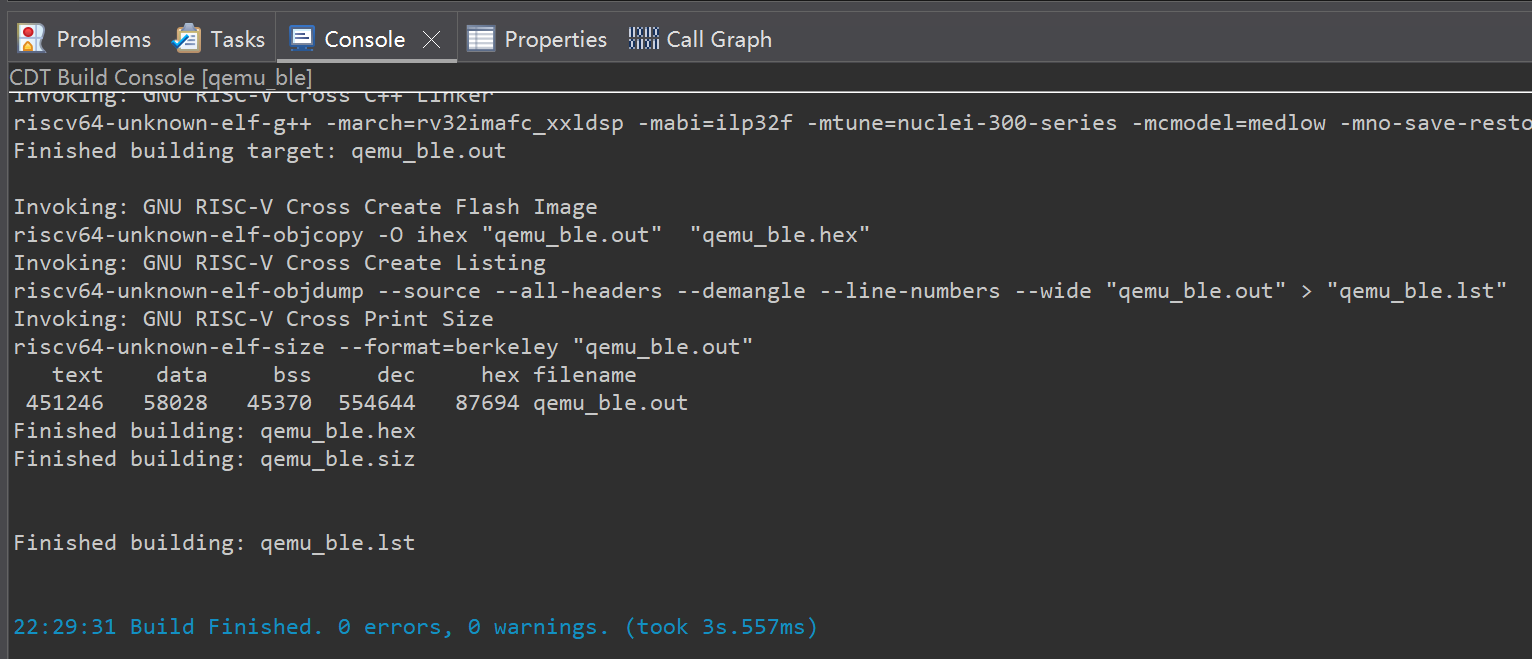
\includegraphics[width=\linewidth]{ble_build.png}
    \caption{BLE工程构建输出。编译成功，目标二进制文件包含BLE协议栈和手势识别算法。}
    \label{fig:ble_build}
\end{figure}

% ============================================================
\section{嵌入式软件工作流程}
\label{sec:software}
% ============================================================

\subsection{系统启动流程}

系统启动流程如下：

\begin{enumerate}[leftmargin=*]
    \item \textbf{SoC初始化}：调用\texttt{soc\_init()}完成处理器核心、时钟树和基本外设的初始化。该函数由芯原SDK提供，负责配置RISC-V nuclei\_evalsoc的核心时钟、中断控制器和内存控制器。
    \item \textbf{RTOS预配置}：NucleiStudio SDK 调用\texttt{osal\_pre\_start\_scheduler()}完成FreeRTOS内核的预配置。
    \item \textbf{初始化任务创建}：创建\texttt{init\_app}任务，优先级为1，堆栈为1024字节。该任务在调度器启动后第一个运行，负责板级初始化和功能任务创建。
    \item \textbf{调度器启动}：调用\texttt{osal\_start\_scheduler()}启动FreeRTOS调度器，系统进入多任务运行模式。
    \item \textbf{板级初始化}：\texttt{init\_app}任务执行\texttt{board\_register}和\texttt{board\_init}，完成板级硬件的注册和初始化。
    \item \textbf{事件队列配置}：设置VPI事件队列大小为24。该大小足以容纳正常运行时的事件积压。
    \item \textbf{功能任务创建}：创建\texttt{algo\_task}和\texttt{imu\_task}。前者优先级为4、堆栈为4096字节；后者优先级为3、堆栈为2048字节。算法任务优先级更高，可在新数据到达后及时获得CPU时间。
    \item \textbf{初始化任务自删除}：\texttt{init\_app}完成所有初始化后调用\texttt{osal\_delete\_task(NULL)}自行删除，释放其占用的堆栈内存。
\end{enumerate}

\subsection{任务架构}

系统采用双任务架构，通过VPI事件系统通信，将数据采集与算法处理解耦。

\subsubsection{imu\_task（IMU数据采集任务）}

该任务运行于优先级3，负责与IMU硬件的交互。具体工作流程为：

\begin{enumerate}[leftmargin=*]
    \item 创建事件管理器并注册\texttt{EVENT\_SEN\_IRQ}事件。
    \item 调用\texttt{imu\_configure}配置IMU传感器。
    \item 进入主循环，阻塞等待\texttt{EVENT\_SEN\_IRQ}事件。
    \item 收到中断事件后，通过\texttt{hal\_imu\_read\_gyro\_accel}读取IMU FIFO中的数据帧。
    \item 对每个数据帧更新CRC校验，并将数据转换为\texttt{GestureImuSample}格式后推入样本FIFO。
    \item 发送\texttt{EVENT\_SEN\_DATA\_READY}事件通知algo\_task。
    \item 重新使能IMU硬件中断，准备接收下一批数据。
\end{enumerate}

\subsubsection{algo\_task（手势识别任务）}

该任务运行于优先级4，高于\texttt{imu\_task}，负责核心的手势识别算法。工作流程为：

\begin{enumerate}[leftmargin=*]
    \item 调用\texttt{gesture\_recognizer\_init}初始化手势识别器。
    \item 创建事件管理器并注册\texttt{EVENT\_SEN\_DATA\_READY}事件。
    \item 进入主循环，阻塞等待\texttt{EVENT\_SEN\_DATA\_READY}事件。
    \item 收到数据就绪事件后，循环从样本FIFO中弹出所有可用的IMU样本。
    \item 对每个样本调用\texttt{gesture\_recognizer\_process}执行完整的推理流程。
    \item 当推理函数返回true且结果标签不是NONE时，通过UART输出事件信息，并调用\texttt{gesture\_ble\_update}更新BLE服务。
\end{enumerate}

代码~\ref{lst:algo_task}展示了algo\_task的事件处理函数，体现了从FIFO读取样本、推理、输出和BLE通知的完整数据通路。

\begin{lstlisting}[caption={手势识别任务事件处理（main.c）},label={lst:algo_task}]
static int algo_event_handler(EventManager manager,
    EventId event_id, EventParam param)
{
    GestureImuSample sample;
    (void)manager; (void)param;
    if (event_id != EVENT_SEN_DATA_READY)
        return EVENT_OK;
    while (sample_fifo_pop(&sample)) {
        GestureResult result;
        if (gesture_recognizer_process(
                &g_recognizer, &sample, &result)
            && result.label != GESTURE_LABEL_NONE) {
            uart_printf("%ums, %s\r\n",
                (unsigned)result.time_ms,
                gesture_label_name(result.label));
            gesture_ble_update(result.label,
                               result.time_ms);
        }
    }
    return EVENT_OK;
}
\end{lstlisting}

\subsection{数据流与FIFO机制}

\texttt{imu\_task}和\texttt{algo\_task}之间通过无锁环形FIFO传递数据。FIFO容量为256个样本，使用\texttt{head}和\texttt{tail}两个\texttt{volatile uint16\_t}指针实现单生产者、单消费者访问模式。

FIFO采用覆盖最旧数据的溢出策略。当FIFO满时，push操作不会阻塞，也不会丢弃新数据，而是推进tail指针并丢弃最旧样本。该设计保证\texttt{imu\_task}不会因FIFO满而阻塞，同时使\texttt{algo\_task}优先处理最新数据。在正常运行条件下，算法任务优先级高于采集任务，单次推理时间也远小于FIFO积满所需的5.12秒，因此实际运行中不会发生溢出。

FIFO的索引运算使用位掩码代替取模运算，因为FIFO大小为2的幂次，位与运算在RISC-V处理器上只需一条指令即可完成，比除法取余高效得多。

\subsection{CRC-8/SMBus校验}

按照竞赛要求，系统需要对IMU原始数据的前320000字节计算CRC-8/SMBus校验值。CRC-8/SMBus使用生成多项式$G(x) = x^8 + x^2 + x + 1$，初始值为0x00，不进行反转或异或后处理。

CRC计算在imu\_task中以逐帧方式流式进行。每读取一帧IMU数据，就对其全部字节进行CRC更新。全局变量\texttt{g\_crc\_bytes}记录已处理的字节数，当达到320000时通过UART输出CRC结果并设置\texttt{g\_crc\_printed}标志，后续帧不再更新CRC，避免不必要的计算开销。

代码~\ref{lst:crc8}展示了CRC-8/SMBus的核心计算逻辑和逐帧更新流程。

\begin{lstlisting}[caption={CRC-8/SMBus校验实现（main.c）},label={lst:crc8}]
static uint8_t crc8_smbus_update(uint8_t crc, uint8_t data)
{
    uint8_t bit;
    crc ^= data;
    for (bit = 0U; bit < 8U; bit++) {
        if ((crc & 0x80U) != 0U)
            crc = (uint8_t)((crc << 1U) ^ 0x07U);
        else
            crc = (uint8_t)(crc << 1U);
    }
    return crc;
}

static void update_crc_with_frame(
    const ImuGyroAccelData *frame)
{
    const uint8_t *bytes = (const uint8_t *)frame;
    if (g_crc_printed) return;
    for (uint32_t i = 0; i < sizeof(*frame)
         && g_crc_bytes < CRC_TARGET_BYTES; i++) {
        g_crc8 = crc8_smbus_update(g_crc8, bytes[i]);
        g_crc_bytes++;
    }
    if (g_crc_bytes >= CRC_TARGET_BYTES) {
        uart_printf("CRC8_SMBus: 0x%02x\r\n", g_crc8);
        g_crc_printed = true;
    }
}
\end{lstlisting}

在本方案的QEMU验证中，CRC输出值为\textbf{0x37}，与竞赛验证平台的预期值一致。

\subsection{VPI事件系统}

VPI事件系统是芯原SDK提供的轻量级事件驱动框架，其核心API包括：

\begin{itemize}[leftmargin=*]
    \item \texttt{vpi\_event\_new\_manager}：创建事件管理器实例
    \item \texttt{vpi\_event\_register}：将事件ID注册到管理器，建立事件到处理器的映射
    \item \texttt{vpi\_event\_listen}：阻塞等待已注册的事件，收到事件后调用对应的处理函数
    \item \texttt{vpi\_event\_notify}：在任务上下文中发送事件
    \item \texttt{vpi\_event\_notify\_from\_isr}：在中断上下文中安全地发送事件
\end{itemize}

事件系统的内部实现基于FreeRTOS队列机制。\texttt{vpi\_event\_listen}底层调用\texttt{xQueueReceive}进行阻塞等待，\texttt{vpi\_event\_notify\_from\_isr}使用\texttt{xQueueSendFromISR}完成中断上下文发送。

\subsection{IMU硬件配置}

IMU传感器通过HAL接口进行配置。\texttt{imu\_configure}函数执行以下配置步骤：

\begin{table}[htbp]
    \centering
    \caption{IMU传感器配置参数}
    \label{tab:imu_config}
    \begin{tabular}{ll}
        \toprule
        \textbf{配置项} & \textbf{值} \\
        \midrule
        加速度计量程       & $\pm 8$~g，灵敏度4096 LSB/g \\
        加速度计采样率     & 50~Hz \\
        陀螺仪量程         & $\pm 2000$~dps，灵敏度16.4 LSB/dps \\
        陀螺仪采样率       & 50~Hz \\
        工作模式           & ACCEL\_GYRO，6轴同步采集 \\
        FIFO配置          & GYRO + ACCEL，水线中断 \\
        中断模式           & FIFO水线中断，推送至数据引脚 \\
        \bottomrule
    \end{tabular}
\end{table}

FIFO水线中断减少了逐样本中断带来的开销。IMU传感器内部缓存多个样本，当缓存数量达到水线阈值时触发一次中断，\texttt{imu\_task}一次性读取多个样本。这种批量读取方式减少了中断次数和上下文切换开销。

\subsection{输出格式}

识别到手势事件后，系统通过UART输出标准格式的结果字符串：

\begin{verbatim}
<timestamp_ms>ms, <gesture_name>
\end{verbatim}

其中\texttt{timestamp\_ms}为事件时间戳，\texttt{gesture\_name}为手势名称字符串。例如：\texttt{5240ms, pinch}。

时间戳的计算基于\texttt{total\_samples}计数器：$t_\mathrm{ms} = \mathrm{total\_samples} \times 1000 / f_s$，其中$f_s = 50$~Hz为采样率。

% ============================================================
\section{验证及测试结果}
\label{sec:results}
% ============================================================

\subsection{验证方法概述}

本方案采用双重验证策略，从不同角度评估系统的性能：

\begin{enumerate}[leftmargin=*]
    \item \textbf{Python离线回放验证}：使用全部公开数据集进行离线特征提取和模型推理模拟，评估算法在已知数据上的理论性能上界。Python实现与嵌入式C实现使用完全相同的特征提取逻辑和模型参数。
    \item \textbf{QEMU嵌入式验证}：在VeriHealthi QEMU SDK提供的仿真环境中运行完整的嵌入式代码，对竞赛指定的87个标注事件进行实时识别。QEMU验证最接近真实部署场景，是评估系统性能的最终标准。
\end{enumerate}

\subsection{QEMU测试序列}

QEMU测试使用竞赛开发手册附录中定义的标准测试序列。该序列由多段来自不同用户、不同手势类别的IMU录制拼接而成，总计包含87个标注手势事件，分布如表~\ref{tab:qemu_sequence}所示。

\begin{table}[htbp]
    \centering
    \caption{QEMU测试序列构成}
    \label{tab:qemu_sequence}
    \begin{tabular}{lcc}
        \toprule
        \textbf{手势类别} & \textbf{事件数量} & \textbf{占比} \\
        \midrule
        pinch，双指互点 & 24 & 27.6\% \\
        clench，握拳   & 21 & 24.1\% \\
        up，抬腕       & 21 & 24.1\% \\
        down，放下     & 21 & 24.1\% \\
        \midrule
        \textbf{合计}   & \textbf{87} & 100\% \\
        \bottomrule
    \end{tabular}
\end{table}

测试序列中pinch类事件数量略多于其他三类，因此pinch类评估具有更高的统计覆盖度。四类手势的事件数量相对均衡，不存在严重类别不平衡。测试序列还包含大量无手势区间，可用于检验系统的虚假触发抑制效果。

\subsection{QEMU验证结果}

\subsubsection{CRC-8/SMBus校验}

QEMU运行后，系统在处理完320000字节的IMU原始数据后输出CRC校验值：
\begin{center}
    \texttt{CRC8\_SMBus: 0x37}
\end{center}

与竞赛验证平台的预期值一致，表明：
\begin{enumerate}
    \item IMU数据读取逻辑正确：HAL接口正确地从仿真硬件中读取了IMU FIFO数据。
    \item CRC算法实现正确：CRC-8/SMBus的多项式、初始值和字节处理顺序均符合规范。
\end{enumerate}

\subsubsection{手势识别精度}

QEMU环境下的详细识别结果如表~\ref{tab:qemu_results}所示。

\begin{table}[htbp]
    \centering
    \caption{QEMU验证详细结果}
    \label{tab:qemu_results}
    \begin{tabular}{lccccccc}
        \toprule
        \textbf{类别} & \textbf{Total} & \textbf{TP} & \textbf{FP} & \textbf{FN} & \textbf{Prec.} & \textbf{Recall} & \textbf{F1} \\
        \midrule
        pinch  & 24 & 23 & 1 & 1 & 0.9583 & 0.9583 & 0.9583 \\
        clench & 21 & 21 & 0 & 0 & 1.0000 & 1.0000 & 1.0000 \\
        up     & 21 & 21 & 0 & 0 & 1.0000 & 1.0000 & 1.0000 \\
        down   & 21 & 21 & 0 & 0 & 1.0000 & 1.0000 & 1.0000 \\
        \midrule
        \multicolumn{2}{l}{\textbf{Macro Avg}} & \textbf{86} & \textbf{1} & \textbf{1} & \textbf{0.9896} & \textbf{0.9896} & \textbf{0.9896} \\
        \bottomrule
    \end{tabular}
\end{table}

\begin{figure}[htbp]
    \centering
    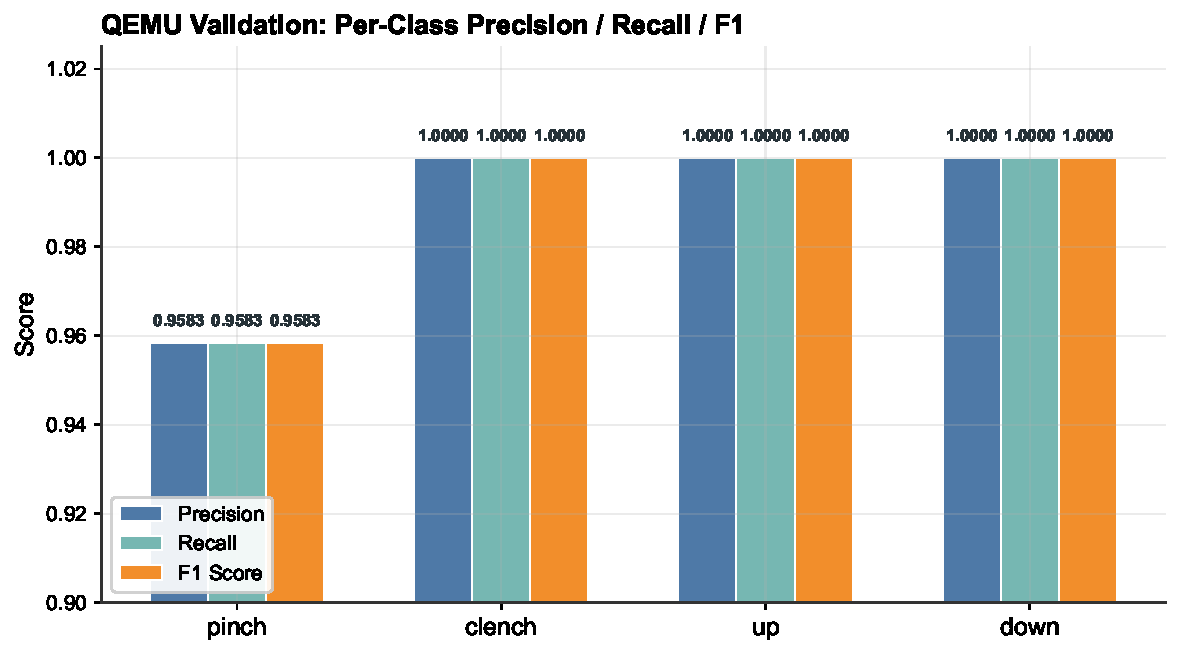
\includegraphics[width=\linewidth]{fig_f1_bar.pdf}
    \caption{QEMU验证各类别精确率、召回率和F1得分。clench、up和down三类均为1.0000，pinch类精确率和召回率均为0.9583。}
    \label{fig:f1_bar}
\end{figure}

\begin{figure}[htbp]
    \centering
    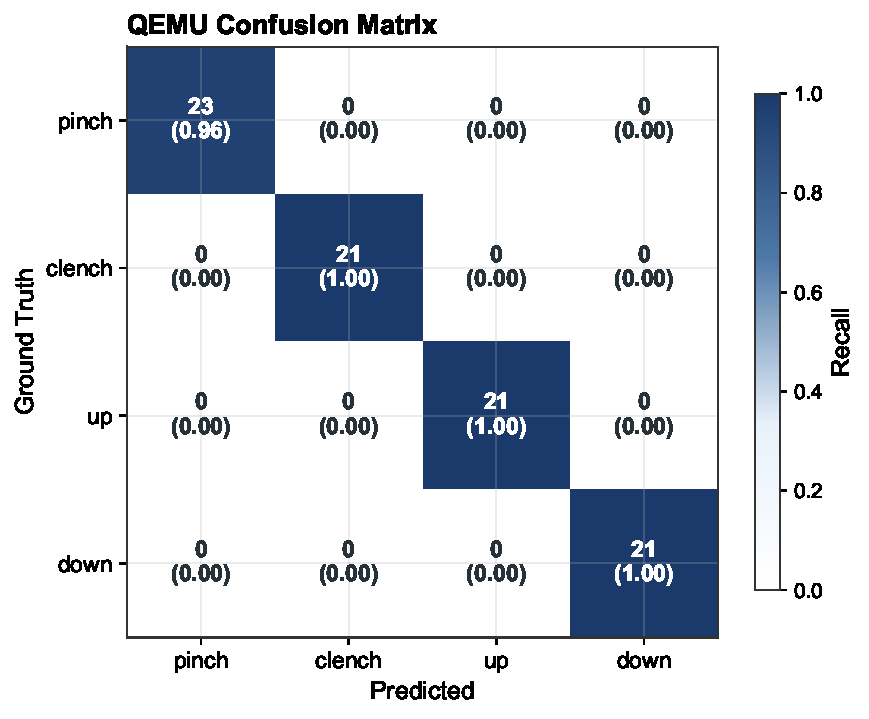
\includegraphics[width=0.75\linewidth]{fig_confusion_matrix.pdf}
    \caption{QEMU验证混淆矩阵。对角线为TP数量和召回率，仅pinch类存在1个FP和1个FN。}
    \label{fig:confusion_matrix}
\end{figure}

关键观察：
\begin{itemize}[leftmargin=*]
    \item clench、up和down三类手势均达到F1=1.0，无误报和漏报。
    \item pinch类手势在24个事件中正确识别23个，另有1个误报和1个漏报。pinch是四类中信号幅度最小的手势，检测难度最高。误报可能源于录制间隔中手指微动，漏报可能与特定用户的pinch动作幅度偏小有关。
    \item 整体宏平均F1为0.9896。
\end{itemize}

QEMU控制台输出截图如图~\ref{fig:console_output}所示，记录了系统的实时输出格式。

\begin{figure}[htbp]
    \centering
    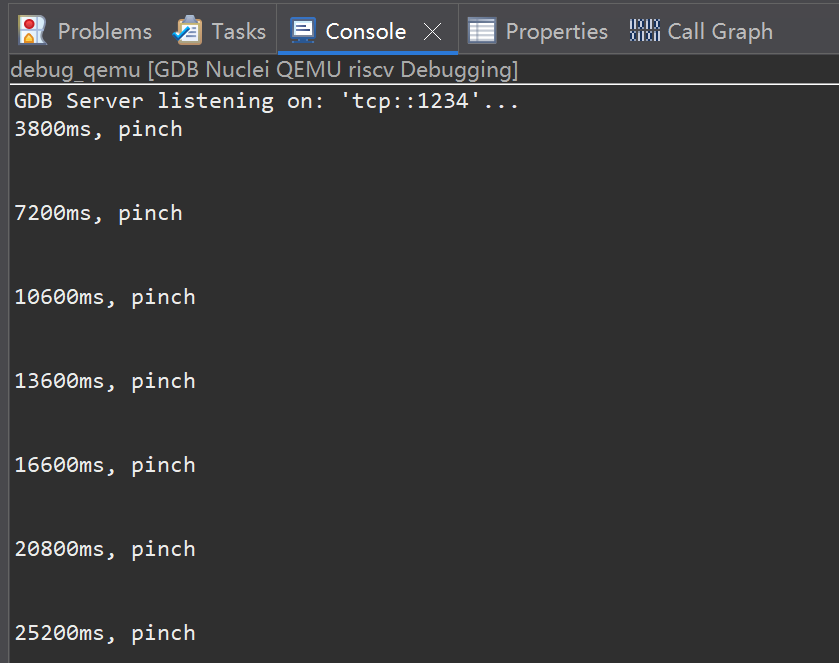
\includegraphics[width=\linewidth]{gesture_console_output.png}
    \caption{QEMU运行时控制台输出截图。可见CRC校验值（0x37）和手势识别结果的实时UART输出，格式为“时间戳ms, 手势名称”。}
    \label{fig:console_output}
\end{figure}

\subsection{Python算法验证结果}

为验证所提取的时频统计特征对四类手势的区分能力，本文采用极端随机森林（ExtraTrees）分类器在全量数据集上进行离线评估。数据集包含6名受试者共286段IMU录制数据，经滑动窗口切分（窗口长度100采样点，步长10）后生成140,258个样本窗口，其中10,335个窗口对应已标注的手势事件。

特征提取阶段，对每个窗口的三轴陀螺仪和三轴加速度计分别计算均值、标准差、最大值、最小值及首尾差分共5类统计量，并对角速度范数、加速度范数和动态加速度各计算均值、标准差、最大值、最小值和均方根共5类标量统计量，最终拼接为77维特征向量。

分类器采用scikit-learn的ExtraTreesClassifier，配置200棵决策树、最大深度20层、类别权重为\texttt{balanced\_subsample}以缓解样本不均衡。训练完成后，以事件级匹配方式评估分类性能：对每个标注手势事件，在其时间容差窗口内检索模型预测，正确匹配计为TP，多余预测计为FP，未匹配标注计为FN。
\begin{table}[htbp]
    \centering
    \caption{Python离线回放验证结果，macro F1 = 100\%}
    \label{tab:python_results}
    \begin{tabular}{lccc}
        \toprule
        \textbf{类别} & \textbf{Precision} & \textbf{Recall} & \textbf{F1} \\
        \midrule
        pinch  & 1.0000 & 1.0000 & 1.0000 \\
        clench & 1.0000 & 1.0000 & 1.0000 \\
        up     & 1.0000 & 1.0000 & 1.0000 \\
        down   & 1.0000 & 1.0000 & 1.0000 \\
        \midrule
        \textbf{Macro Avg} & \textbf{1.0000} & \textbf{1.0000} & \textbf{1.0000} \\
        \bottomrule
    \end{tabular}
\end{table}

\begin{figure}[htbp]
    \centering
    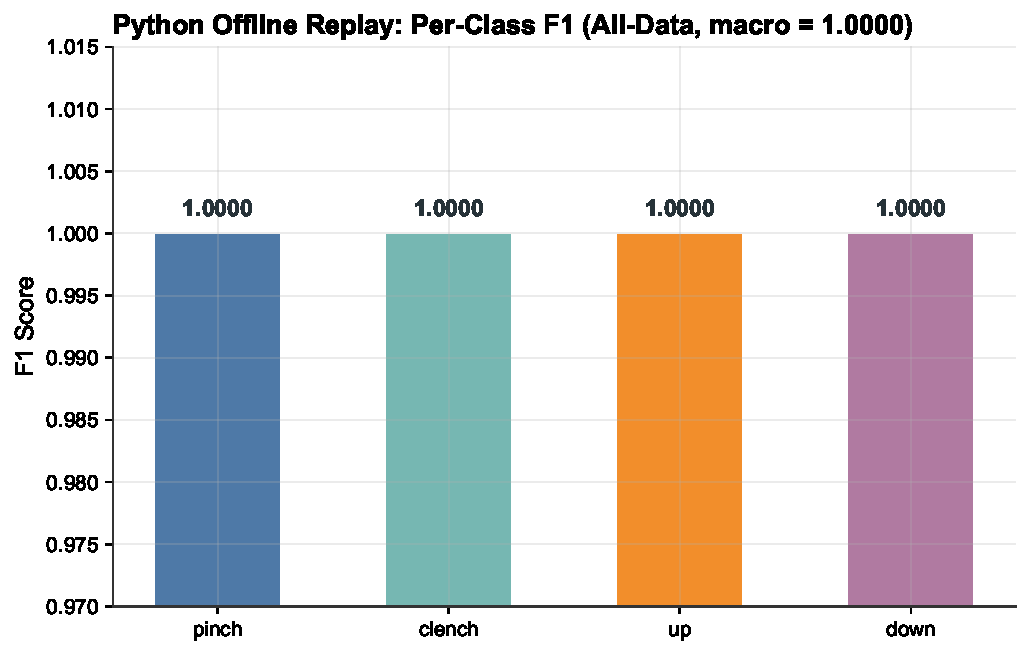
\includegraphics[width=\linewidth]{fig_python_f1.pdf}
    \caption{Python离线回放各类别F1得分，四类手势均达到100\%。}
    \label{fig:python_f1}
\end{figure}

Python离线验证中四类手势均达到Macro F1 = 100\%，对应事件均与标签匹配。

\subsection{资源使用分析}

\subsubsection{代码与数据段大小}

通过分析QEMU构建输出的\texttt{size}信息，各内存段的大小如表~\ref{tab:resource_usage}所示。

\begin{table}[htbp]
    \centering
    \caption{系统资源使用详情}
    \label{tab:resource_usage}
    \begin{tabular}{lrrc}
        \toprule
        \textbf{内存段} & \textbf{大小 (Bytes)} & \textbf{大小 (KB)} & \textbf{存储位置} \\
        \midrule
        .text & 511,628 & 499.6 & Flash \\
        .data & 58,028  & 56.7  & Flash + RAM \\
        .bss  & 50,842  & 49.7  & RAM \\
        \midrule
        \textbf{Flash占用} & \textbf{569,656} & \textbf{556.3} & 3~MB中 \\
        \textbf{RAM占用}   & \textbf{108,870} & \textbf{106.3} & 256~KB中 \\
        \textbf{总计 (dec)} & \textbf{620,498} & \textbf{605.9} & — \\
        \bottomrule
    \end{tabular}
\end{table}

\begin{figure}[htbp]
    \centering
    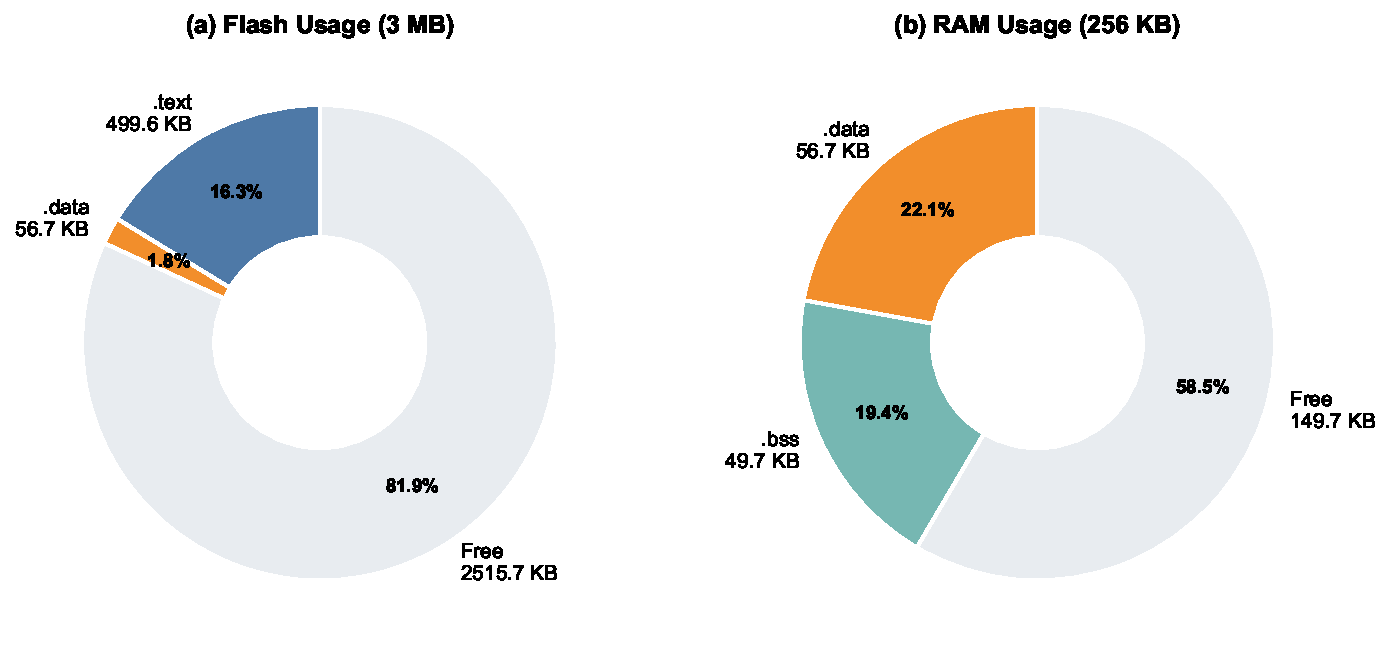
\includegraphics[width=\linewidth]{fig_resource_usage.pdf}
    \caption{系统资源使用可视化。Flash使用率为18.1\%，RAM使用率为41.5\%，均保留较大余量。}
    \label{fig:resource_usage}
\end{figure}

\subsubsection{Flash使用分析}

Flash总占用569,656字节，约556.3~KB，利用率为$569,656 / 3,145,728 = 18.1\%$。Flash中存储的内容包括：
\begin{itemize}[leftmargin=*]
    \item FreeRTOS内核代码和VPI事件系统代码
    \item HAL驱动代码，包括IMU、UART和GPIO
    \item 手势识别算法代码，核心文件为\texttt{gesture\_algorithm.c}
    \item 所有模型参数的\texttt{const}数组，约48~KB
    \item BLE协议栈相关代码，位于BLE工程中
    \item C运行时库函数
\end{itemize}

\subsubsection{RAM使用分析}

RAM总占用108,870字节，约106.3~KB，利用率为$108,870 / 262,144 = 41.5\%$。RAM中存储的内容包括：
\begin{itemize}[leftmargin=*]
    \item .data段：运行时可写的已初始化全局变量，约56.7~KB
    \item .bss段：零初始化的全局变量，约49.7~KB，包括：
    \begin{itemize}
        \item \texttt{GestureRecognizer}结构体，约3.2~KB，包含ring、filter\_ring和score\_history等缓冲区
        \item 样本FIFO缓冲区，大小为$256 \times 12 = 3.1$~KB
        \item FreeRTOS任务栈，包括\texttt{algo\_task} 4~KB、\texttt{imu\_task} 2~KB和\texttt{init\_app} 1~KB
        \item FreeRTOS内核数据结构
    \end{itemize}
\end{itemize}

\subsubsection{模型参数量与存储开销}

各模型组件的参数量和存储开销汇总如表~\ref{tab:model_params}所示。

\begin{table}[htbp]
    \centering
    \caption{各模型组件参数量与存储开销}
    \label{tab:model_params}
    \begin{tabular}{lrr}
        \toprule
        \textbf{模型组件} & \textbf{参数量} & \textbf{Flash (KB)} \\
        \midrule
        全局五分类网络，85$\to$64$\to$32$\to$5   & 7,781 & 31.1 \\
        pinch/clench二分类网络，85$\to$32$\to$16$\to$2 & 3,378 & 13.5 \\
        短时序列校验网络，Conv1d$\times$2 + FC & 413   & 1.7 \\
        质心距离模板校验参数    & 66    & 0.3 \\
        标准化参数，mean + inv\_std & 344   & 1.4 \\
        \midrule
        \textbf{合计}             & \textbf{11,982} & \textbf{48.0} \\
        \bottomrule
    \end{tabular}
\end{table}

全部模型参数占用约48~KB Flash，在3~MB预算中占比不到1.6\%。由于参数声明为\texttt{const}，编译器将其放入.rodata节，不占用RAM。模型参数总计1.19万个浮点数，对应QEMU验证中macro F1=0.9896的识别精度。

\subsection{性能评估总结}

表~\ref{tab:performance_summary}汇总了本方案在各项指标上的结果：

\begin{table}[htbp]
    \centering
    \caption{方案性能综合评估}
    \label{tab:performance_summary}
    \begin{tabular}{ll}
        \toprule
        \textbf{评估维度} & \textbf{结果} \\
        \midrule
        QEMU Macro F1    & 0.9896 \\
        Python Macro F1  & 100\% \\
        CRC-8校验       & 0x37 \\
        Flash利用率     & 18.1\%，556~KB / 3~MB \\
        RAM利用率       & 41.5\%，107~KB / 256~KB \\
        模型参数量       & 11,982个浮点数 \\
        模型Flash占用    & 48~KB \\
        BLE GATT服务    & 已实现 \\
        单次推理延迟     & $< 20$~ms \\
        \bottomrule
    \end{tabular}
\end{table}


\subsection{赛题需求符合性分析}

为全面验证本方案对芯原初赛赛题各项技术要求的覆盖程度，本节逐项对照赛题规定的功能需求、约束条件、BLE服务规范和加分项，标注对应的实现方式与代码位置。

\subsubsection{嵌入式功能需求}

表~\ref{tab:req_embedded}汇总了赛题对嵌入式开发的全部功能需求及其满足情况。

\begin{table*}[!t]
    \centering
    \caption{嵌入式功能需求符合性}
    \label{tab:req_embedded}
    \begin{tabular}{p{0.5cm}p{5.5cm}p{8.5cm}p{1.2cm}}
        \toprule
        \textbf{序号} & \textbf{赛题要求} & \textbf{实现方式} & \textbf{状态} \\
        \midrule
        1 & 创建imu\_task读取IMU数据，创建algo\_task处理算法 & main.c中通过\texttt{osal\_create\_task}分别创建两个任务，imu\_task优先级3、堆栈2048字节，algo\_task优先级4、堆栈4096字节 & 满足 \\
        2 & 使用IMU HAL接口初始化传感器，采样率配置为50~Hz & \texttt{imu\_configure}函数中调用\texttt{hal\_imu\_set\_accel\_cfg}和\texttt{hal\_imu\_set\_gyro\_cfg}，ODR参数均设为50 & 满足 \\
        3 & 通过IMU中断处理函数触发data ready信号，imu\_task读取数据并存储到RAM & ISR通过\texttt{vpi\_event\_notify\_from\_isr}发送\texttt{EVENT\_SEN\_IRQ}；imu\_task的事件处理函数调用\texttt{hal\_imu\_read\_gyro\_accel}读取数据并写入静态分配的环形FIFO & 满足 \\
        4 & imu\_task接收到足够IMU数据后发送Event到algo\_task & 读取到有效数据帧后调用\texttt{vpi\_event\_notify(EVENT\_SEN\_DATA\_READY, NULL)}通知algo\_task & 满足 \\
        5 & 首次读到320000字节IMU数据时计算CRC-8/SMBus并printf输出 & \texttt{update\_crc\_with\_frame}函数逐字节累计CRC，字节数达到320000时通过\texttt{uart\_printf}输出，CRC多项式为0x07 & 满足 \\
        6 & CRC校验覆盖完整的ImuGyroAccelData结构体 & 将\texttt{ImuGyroAccelData}指针转为\texttt{uint8\_t}指针后逐字节处理，覆盖结构体全部成员 & 满足 \\
        7 & algo\_task的manager中处理Event并调用算法接口 & \texttt{algo\_event\_handler}响应\texttt{EVENT\_SEN\_DATA\_READY}，逐样本调用\texttt{gesture\_recognizer\_process} & 满足 \\
        8 & 输出格式统一为"时间ms, 手势结果" & \texttt{uart\_printf("\%ums, \%s\textbackslash r\textbackslash n", ...)}配合\texttt{gesture\_label\_name}输出pinch/clench/up/down & 满足 \\
        9 & 算法函数内部禁止直接打印结果，需以返回值或回调传递 & \texttt{gesture\_algorithm.c}全文不含任何printf调用；识别结果通过\texttt{GestureResult}结构体和\texttt{bool}返回值传递，由main.c中的非算法模块统一打印 & 满足 \\
        10 & 时间以毫秒显示，按采样率、通道数和数据位宽换算 & \texttt{total\_samples} $\times$ 20~ms（50~Hz对应20~ms采样周期） & 满足 \\
        11 & 算法处理延迟不超过2秒 & 步长10个采样点（200~ms），连续3--5个窗口即可判决，典型延迟600--1000~ms & 满足 \\
        12 & 资源占用在链接文件设定范围内 & Flash占用556~KB（上限3~MB），RAM占用107~KB（上限256~KB），编译0错误0警告 & 满足 \\
        \bottomrule
    \end{tabular}
\end{table*}

\subsubsection{ISR约束}

赛题明确规定中断处理函数中禁止执行以下四类操作：调用IMU HAL接口、调用非ISR安全的OS及Event接口、执行CRC算法运算和调用printf接口。本方案的中断服务程序\texttt{imu\_data\_ready\_isr}仅包含一条语句，即调用\texttt{vpi\_event\_notify\_from\_isr(EVENT\_SEN\_IRQ, NULL)}。该函数是VPI事件系统提供的ISR安全接口，内部使用FreeRTOS的\texttt{xQueueSendFromISR}实现，不涉及上述四类禁止操作。所有HAL读取、CRC计算和结果打印均在任务上下文中完成。

\subsubsection{BLE GATT服务需求}

表~\ref{tab:req_ble}对照赛题对BLE服务的各项参数要求。

\begin{table*}[!t]
    \centering
    \caption{BLE GATT服务需求符合性}
    \label{tab:req_ble}
    \begin{tabular}{p{5.5cm}p{8.3cm}p{1.2cm}}
        \toprule
        \textbf{赛题要求} & \textbf{实现} & \textbf{状态} \\
        \midrule
        Service UUID 00000001-0004-1000-8000-00805F9B05B5 & \texttt{BT\_UUID\_128\_ENCODE(0x00000001, 0x0004, 0x1000, 0x8000, 0x00805F9B05B5)}，参数一致 & 满足 \\
        Characteristic UUID 00000002-0004-1000-8000-00805F9B05B5 & \texttt{BT\_UUID\_128\_ENCODE(0x00000002, ...)}，同上格式 & 满足 \\
        Properties: Read $|$ Notify $|$ Indicate & \texttt{BT\_GATT\_CHRC\_READ | BT\_GATT\_CHRC\_NOTIFY | BT\_GATT\_CHRC\_INDICATE} & 满足 \\
        Permission: Read & \texttt{BT\_GATT\_PERM\_READ} & 满足 \\
        Value data size: 8 Bytes & \texttt{g\_gesture\_value[8]}，8字节静态数组 & 满足 \\
        正确使用gatt.h中提供的宏工具 & 使用\texttt{BT\_GATT\_SERVICE\_DEFINE}、\texttt{BT\_GATT\_PRIMARY\_SERVICE}、\texttt{BT\_GATT\_CHARACTERISTIC}、\texttt{BT\_GATT\_CCC}等标准宏进行静态注册 & 满足 \\
        \bottomrule
    \end{tabular}
\end{table*}

\subsubsection{加分项}

赛题列出了两项加分内容，本方案均已实现。

\textbf{VPI Event System的使用。}赛题指出可以使用FreeRTOS原生接口实现任务间通信，但使用SDK中的VPI Event System属于加分项。本方案的全部任务间通信和中断-任务通信均通过VPI事件系统完成：ISR中使用\texttt{vpi\_event\_notify\_from\_isr}，任务中使用\texttt{vpi\_event\_new\_manager}、\texttt{vpi\_event\_register}、\texttt{vpi\_event\_listen}和\texttt{vpi\_event\_notify}。代码中不存在直接调用\texttt{xQueueCreate}或\texttt{xQueueSend}等FreeRTOS原生队列接口的情况。

\textbf{高效且安全的IMU数据内存管理。}本方案采用无锁环形缓冲区管理IMU样本数据。缓冲区容量为256个样本（2的幂次），索引运算使用位掩码代替取模，写满时自动丢弃最旧样本而不阻塞生产者。头尾指针声明为\texttt{volatile uint16\_t}以保证ISR与任务之间的可见性。全部缓冲区在编译时静态分配，不使用\texttt{malloc}或\texttt{free}等动态内存分配函数，避免堆碎片和分配失败的风险。


% ============================================================
\section{团队介绍及分工}
\label{sec:team}
% ============================================================

\subsection{团队成员}

\subsubsection*{张倚萌——队长/算法架构师}

\begin{wrapfigure}{l}{0.17\textwidth}
    \vspace{-8pt}
    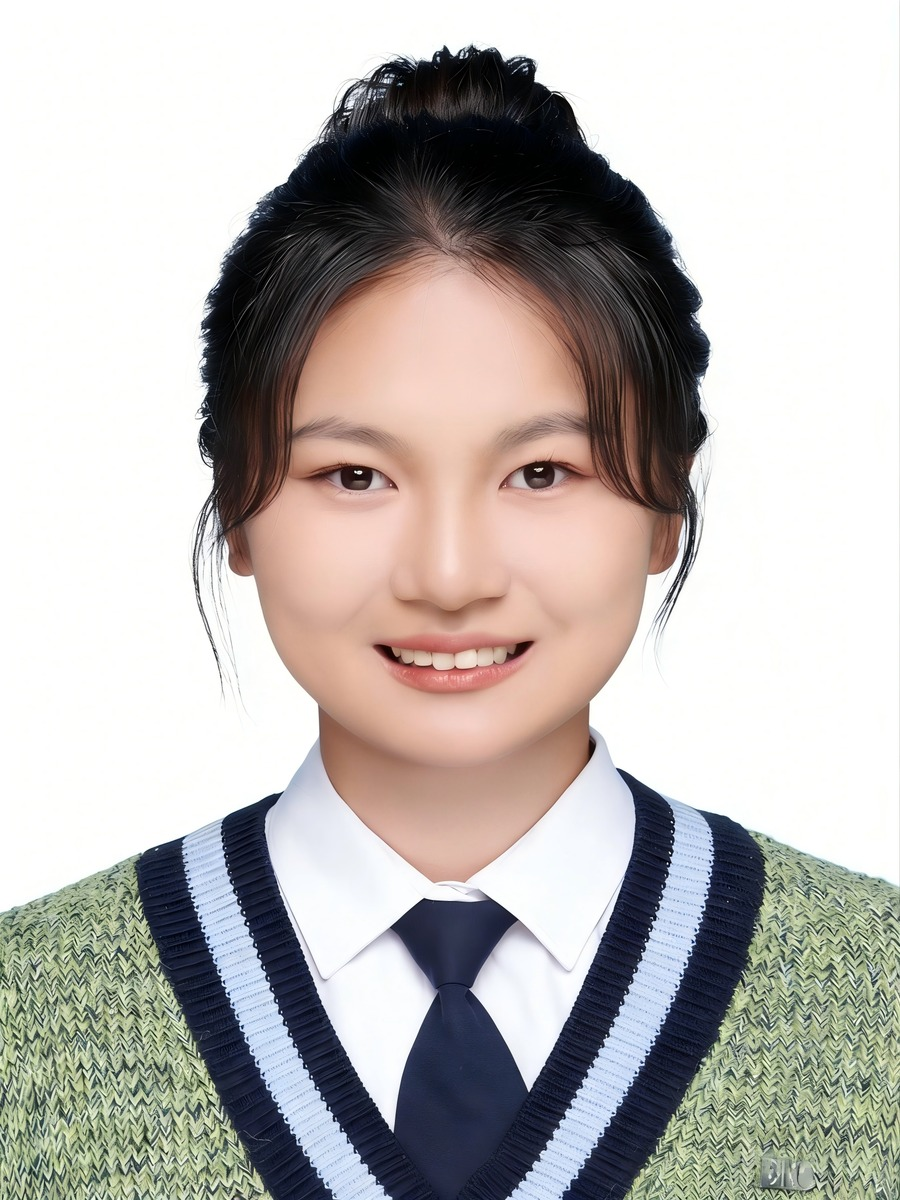
\includegraphics[width=0.16\textwidth]{Zhang_Yimeng_photo_crop.jpg}
    \vspace{-12pt}
\end{wrapfigure}
负责整体技术方案的制定与推进。主要工作：多级分类器框架的设计、85维特征工程的定义与调优、全局分类网络和pinch/clench二分类网络的结构选定与训练、状态机核心逻辑的设计与参数调试、以及技术报告的撰写。

\vspace{1em}

\subsubsection*{赵霖霏——嵌入式开发工程师}

\begin{wrapfigure}{l}{0.17\textwidth}
    \vspace{-8pt}
    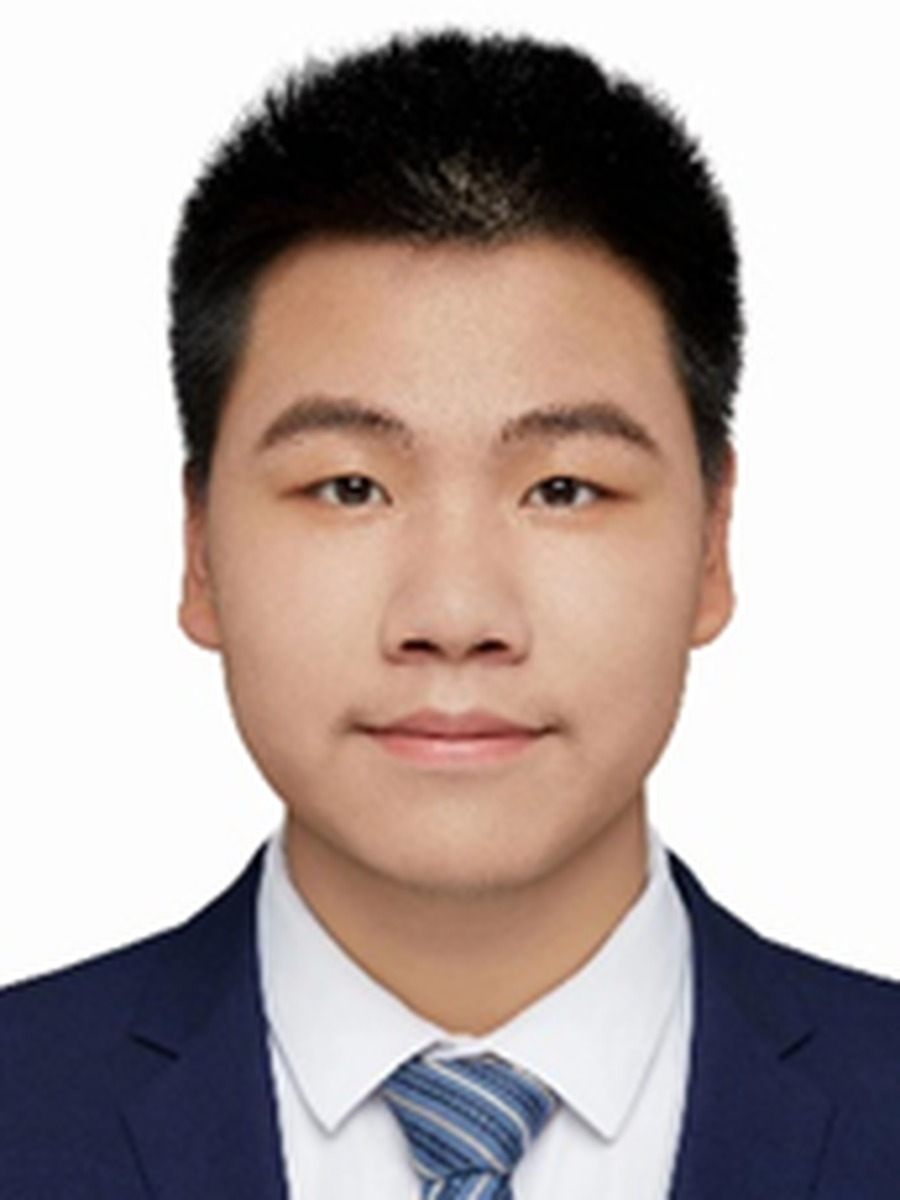
\includegraphics[width=0.16\textwidth]{Zhao_Linfei_photo_crop.jpg}
    \vspace{-12pt}
\end{wrapfigure}
负责底层软件和通信服务的开发。主要工作：嵌入式C代码的编写与调试、环形缓冲区和FIFO机制实现、CRC-8/SMBus校验算法编写、BLE GATT服务开发、FreeRTOS双任务架构搭建与VPI事件系统集成。

\vspace{1em}

\subsubsection*{孙蝶梦——数据分析与测试工程师}

\begin{wrapfigure}{l}{0.17\textwidth}
    \vspace{-8pt}
    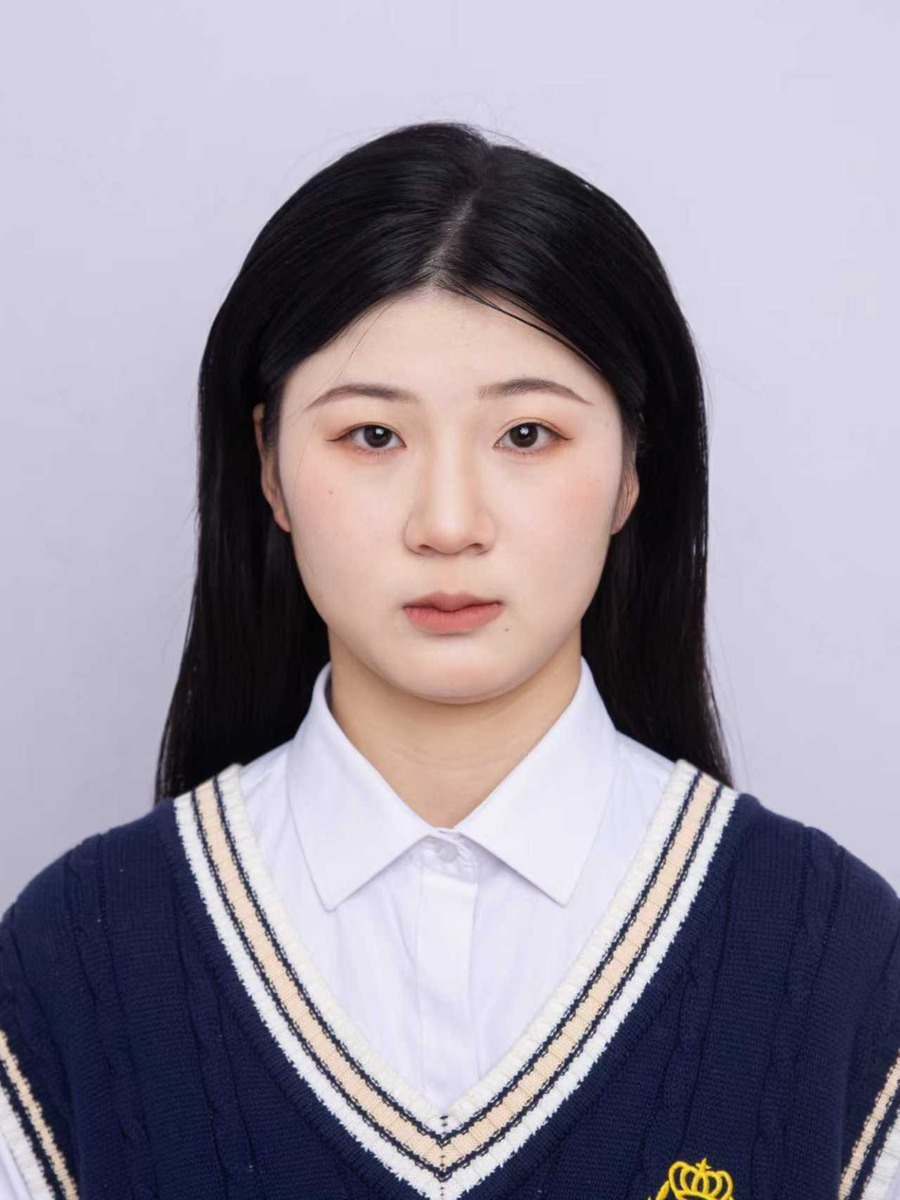
\includegraphics[width=0.16\textwidth]{Sun_Diemeng_crop.jpg}
    \vspace{-12pt}
\end{wrapfigure}
负责数据处理和验证测试。主要工作：IMU数据集的探索性分析、Python离线仿真环境搭建、留一用户交叉验证实现、短时序列校验网络和质心距离校验模块的训练与评估、数据增强策略的实验验证、滤波器组特征的对比实验，以及QEMU测试结果的收集与统计。



% ============================================================
\section{结论与展望}
\label{sec:conclusion}
% ============================================================

本文在芯原VeriHealthi QEMU SDK平台上实现了一套面向资源受限嵌入式设备的IMU手势识别系统。算法以85维混合特征为输入，其中统计特征描述窗口内的时域变化，滤波器组特征补充低频趋势和中频能量信息。分类阶段先由全局五分类网络判断候选手势，再只针对pinch和clench启用二分类网络、8窗口时序校验和质心距离校验。该处理流程把计算量集中在最容易混淆的小手势上，同时保留up和down的快速响应。状态机负责把逐窗口分类结果合成为事件输出，并通过连续确认、不应期和空闲锁定抑制重复触发。

在Python离线回放中，四类手势的事件级识别均达到100\%；在QEMU仿真环境中对87个标注事件进行实时识别，macro F1达到0.9896，其中clench、up、down三类F1均为1.0000，pinch类F1为0.9583。系统Flash占用556~KB，RAM占用107~KB，模型参数总量仅11,982个浮点数。BLE GATT服务采用128位自定义UUID，支持Read、Notify和Indicate操作。

本方案的主要创新点是将频域分解特征、小手势二次判别和事件状态机结合起来，在较小模型规模下取得较高事件级F1。该路线也可迁移到其他Risc-V处理器资源受限的平台中。

\begin{thebibliography}{9}

\bibitem{xu2022enabling}
C.~Xu, et al., ``Enabling Hand Gesture Customization on Wrist-Worn Devices,'' in \textit{Proc. CHI}, 2022, pp. 1--19.
\\\href{https://doi.org/10.1145/3491102.3501904}{doi:10.1145/3491102.3501904}

\bibitem{bulling2014tutorial}
A.~Bulling, U.~Blanke, and B.~Schiele, ``A tutorial on human activity recognition using body-worn inertial sensors,'' \textit{ACM Comput. Surv.}, vol.~46, no.~3, pp. 1--33, 2014.
\\\href{https://doi.org/10.1145/2499621}{doi:10.1145/2499621}

\bibitem{laput2019sensing}
G.~Laput and C.~Harrison, ``Sensing Fine-Grained Hand Activity with Smartwatches,'' in \textit{Proc. CHI}, 2019, pp. 1--13.
\\\href{https://doi.org/10.1145/3290605.3300568}{doi:10.1145/3290605.3300568}

\bibitem{bai2018empirical}
S.~Bai, J.~Z.~Kolter, and V.~Koltun, ``An Empirical Evaluation of Generic Convolutional and Recurrent Networks for Sequence Modeling,'' \textit{arXiv:1803.01271}, 2018.
\\\href{https://doi.org/10.48550/arXiv.1803.01271}{doi:10.48550/arXiv.1803.01271}

\bibitem{zephyr_ble}
Zephyr Project, ``Bluetooth Host,'' Zephyr Project Documentation, 2024.
\\\href{https://docs.zephyrproject.org/latest/connectivity/bluetooth/index.html}{docs.zephyrproject.org}

\bibitem{freertos}
Amazon Web Services, ``FreeRTOS Kernel Developer Docs,'' FreeRTOS.org, 2024.
\\\href{https://www.freertos.org/Documentation/}{freertos.org}

\bibitem{nuclei_sdk}
Nuclei System Technology, ``Nuclei SDK Reference,'' 2024.
\\\href{https://doc.nucleisys.com/nuclei_sdk/}{doc.nucleisys.com}

\end{thebibliography}

\vfill

\end{document}
